\documentclass[12pt]{article}

% Separate working manuscript. Canonical main.* files are unchanged.
% !TEX TS-program = xelatex
% File: preamble.tex
% Purpose: Brett Reynolds house style LaTeX preamble
% Version: 2.0.0 (December 2025 typography redesign)
%
% Usage: % !TEX TS-program = xelatex
% File: preamble.tex
% Purpose: Brett Reynolds house style LaTeX preamble
% Version: 2.0.0 (December 2025 typography redesign)
%
% Usage: % !TEX TS-program = xelatex
% File: preamble.tex
% Purpose: Brett Reynolds house style LaTeX preamble
% Version: 2.0.0 (December 2025 typography redesign)
%
% Usage: \input{.house-style/preamble.tex} in main document
%
% Compiler: XeLaTeX (default) or LuaLaTeX
%           NOT pdfLaTeX - requires fontspec for fonts

% ===========================
% FONTS
% ===========================
\usepackage{fontspec}

\setmainfont{EBGaramond}[
  Extension=.otf,
  UprightFont=*-Regular,
  ItalicFont=*-Italic,
  BoldFont=*-Bold,
  BoldItalicFont=*-BoldItalic,
  Numbers=OldStyle,
  Ligatures=TeX,
]

% IPA fallback font
\newfontfamily\ipafont{CharisSIL}[
  Extension=.ttf,
  UprightFont=*-Regular,
  ItalicFont=*-Italic,
  BoldFont=*-Bold,
  BoldItalicFont=*-BoldItalic,
]
\newcommand{\ipa}[1]{{\ipafont #1}}

% Lining figures when needed (tables, years in isolation)
\providecommand{\liningnums}[1]{{\addfontfeatures{Numbers=Lining}#1}}

% Monospace
\setmonofont{Inconsolatazi4}[
  Extension=.otf,
  UprightFont=*-Regular,
  BoldFont=*-Bold,
  Scale=MatchLowercase,
]

% ===========================
% PAGE LAYOUT
% ===========================
\usepackage[
  letterpaper,
  inner=1.25in,
  outer=1in,
  top=1in,
  bottom=1.25in,
  marginparwidth=0.6in,
]{geometry}

\usepackage[british]{babel}
\usepackage[final]{microtype}

% ===========================
% HEADINGS
% ===========================
\usepackage{titlesec}

% Section: small caps, number in margin
\titleformat{\section}
  {\normalfont\scshape}
  {\llap{\thesection\quad}}
  {0pt}
  {}

% Subsection: small caps sentence case
\titleformat{\subsection}
  {\normalfont\scshape}
  {\thesubsection\quad}
  {0pt}
  {}

% Subsubsection: upright
\titleformat{\subsubsection}
  {\normalfont}
  {\thesubsubsection\quad}
  {0pt}
  {}

% Spacing
\titlespacing*{\section}{0pt}{2ex plus 1ex minus .2ex}{1ex plus .2ex}
\titlespacing*{\subsection}{0pt}{1.5ex plus 1ex minus .2ex}{0.5ex plus .2ex}
\titlespacing*{\subsubsection}{0pt}{1ex plus 0.5ex minus .1ex}{0.3ex plus .1ex}

% ===========================
% RUNNING HEADS
% ===========================
\usepackage{fancyhdr}
\pagestyle{fancy}
\fancyhf{}
\setlength{\headheight}{13.6pt}
\renewcommand{\headrulewidth}{0pt}

% For oneside documents (most papers):
\fancyhead[L]{\small\scshape\leftmark}
\fancyhead[R]{\small\thepage}
\fancyfoot{}

% ===========================
% COLORS & HYPERLINKS
% ===========================
\usepackage{xcolor}
\definecolor{linkmaroon}{RGB}{128, 0, 32}

\usepackage{hyperref}
\hypersetup{
  colorlinks=true,
  linkcolor=linkmaroon,
  citecolor=linkmaroon,
  urlcolor=linkmaroon,
  pdfauthor={Brett Reynolds},
}

\usepackage{orcidlink}

% ===========================
% QUOTATIONS
% ===========================
\usepackage[style=american]{csquotes} % Double quotes outer (Oxford spelling kept via babel)
\MakeOuterQuote{"}

% ===========================
% SEMANTIC MACROS
% ===========================
% Terms (linguistic concepts being introduced/defined)
\newcommand{\term}[1]{\textsc{#1}}

% Mentions (words/expressions under discussion)
\newcommand{\mention}[1]{\textit{#1}}

% Mentions in headings (angle brackets instead of italics)
% Robust: headings are moving arguments (written to .toc/.aux)
\DeclareRobustCommand{\mentionhead}[1]{⟨\textup{#1}⟩}

% Object language (cited forms, foreign words)
\newcommand{\olang}[1]{\textit{#1}}

% Small-caps abbreviations for glosses
\newcommand{\abbr}[1]{\textsc{#1}}

% Cross-linguistic subscript marker
\usepackage{marvosym}
\newcommand{\crossmark}{\textsubscript{\Cross}}

% ===========================
% MATHS AND SYMBOLS
% ===========================
\usepackage{amsmath,amssymb}

% ===========================
% LINGUISTIC EXAMPLES
% ===========================
\usepackage{langsci-gb4e}
\makeatletter
\@ifundefined{noautomath}{}{\noautomath}
\makeatother

% Judgement markers
\newcommand{\ungram}[1]{*\!#1}
\newcommand{\marg}[1]{?\!#1}
\newcommand{\odd}[1]{\#\!#1}

% ===========================
% LISTS
% ===========================
\usepackage{enumitem}
\setlist{nosep, leftmargin=*}
\setlist[enumerate]{label=\arabic*.}
\setlist[itemize]{label=--}

% ===========================
% TABLES & FIGURES
% ===========================
\usepackage{booktabs}
\usepackage{array}
\usepackage{graphicx}
\graphicspath{{figures/}}

% ===========================
% BIBLIOGRAPHY
% ===========================
\usepackage[backend=biber,style=apa,natbib=true,doi=true,isbn=false,url=true]{biblatex}
\addbibresource{references.bib}
\IfFileExists{references-local.bib}{\addbibresource{references-local.bib}}{}

% Possessive citation: Author's (Year)
\newcommand{\posscite}[1]{\citeauthor{#1}'s (\citeyear{#1})}

% ===========================
% UTILITIES
% ===========================
\usepackage{xspace}
\newcommand{\eg}{e.g.,\xspace}
\newcommand{\ie}{i.e.,\xspace}
\newcommand{\etc}{etc.\xspace}
 in main document
%
% Compiler: XeLaTeX (default) or LuaLaTeX
%           NOT pdfLaTeX - requires fontspec for fonts

% ===========================
% FONTS
% ===========================
\usepackage{fontspec}

\setmainfont{EBGaramond}[
  Extension=.otf,
  UprightFont=*-Regular,
  ItalicFont=*-Italic,
  BoldFont=*-Bold,
  BoldItalicFont=*-BoldItalic,
  Numbers=OldStyle,
  Ligatures=TeX,
]

% IPA fallback font
\newfontfamily\ipafont{CharisSIL}[
  Extension=.ttf,
  UprightFont=*-Regular,
  ItalicFont=*-Italic,
  BoldFont=*-Bold,
  BoldItalicFont=*-BoldItalic,
]
\newcommand{\ipa}[1]{{\ipafont #1}}

% Lining figures when needed (tables, years in isolation)
\providecommand{\liningnums}[1]{{\addfontfeatures{Numbers=Lining}#1}}

% Monospace
\setmonofont{Inconsolatazi4}[
  Extension=.otf,
  UprightFont=*-Regular,
  BoldFont=*-Bold,
  Scale=MatchLowercase,
]

% ===========================
% PAGE LAYOUT
% ===========================
\usepackage[
  letterpaper,
  inner=1.25in,
  outer=1in,
  top=1in,
  bottom=1.25in,
  marginparwidth=0.6in,
]{geometry}

\usepackage[british]{babel}
\usepackage[final]{microtype}

% ===========================
% HEADINGS
% ===========================
\usepackage{titlesec}

% Section: small caps, number in margin
\titleformat{\section}
  {\normalfont\scshape}
  {\llap{\thesection\quad}}
  {0pt}
  {}

% Subsection: small caps sentence case
\titleformat{\subsection}
  {\normalfont\scshape}
  {\thesubsection\quad}
  {0pt}
  {}

% Subsubsection: upright
\titleformat{\subsubsection}
  {\normalfont}
  {\thesubsubsection\quad}
  {0pt}
  {}

% Spacing
\titlespacing*{\section}{0pt}{2ex plus 1ex minus .2ex}{1ex plus .2ex}
\titlespacing*{\subsection}{0pt}{1.5ex plus 1ex minus .2ex}{0.5ex plus .2ex}
\titlespacing*{\subsubsection}{0pt}{1ex plus 0.5ex minus .1ex}{0.3ex plus .1ex}

% ===========================
% RUNNING HEADS
% ===========================
\usepackage{fancyhdr}
\pagestyle{fancy}
\fancyhf{}
\setlength{\headheight}{13.6pt}
\renewcommand{\headrulewidth}{0pt}

% For oneside documents (most papers):
\fancyhead[L]{\small\scshape\leftmark}
\fancyhead[R]{\small\thepage}
\fancyfoot{}

% ===========================
% COLORS & HYPERLINKS
% ===========================
\usepackage{xcolor}
\definecolor{linkmaroon}{RGB}{128, 0, 32}

\usepackage{hyperref}
\hypersetup{
  colorlinks=true,
  linkcolor=linkmaroon,
  citecolor=linkmaroon,
  urlcolor=linkmaroon,
  pdfauthor={Brett Reynolds},
}

\usepackage{orcidlink}

% ===========================
% QUOTATIONS
% ===========================
\usepackage[style=american]{csquotes} % Double quotes outer (Oxford spelling kept via babel)
\MakeOuterQuote{"}

% ===========================
% SEMANTIC MACROS
% ===========================
% Terms (linguistic concepts being introduced/defined)
\newcommand{\term}[1]{\textsc{#1}}

% Mentions (words/expressions under discussion)
\newcommand{\mention}[1]{\textit{#1}}

% Mentions in headings (angle brackets instead of italics)
% Robust: headings are moving arguments (written to .toc/.aux)
\DeclareRobustCommand{\mentionhead}[1]{⟨\textup{#1}⟩}

% Object language (cited forms, foreign words)
\newcommand{\olang}[1]{\textit{#1}}

% Small-caps abbreviations for glosses
\newcommand{\abbr}[1]{\textsc{#1}}

% Cross-linguistic subscript marker
\usepackage{marvosym}
\newcommand{\crossmark}{\textsubscript{\Cross}}

% ===========================
% MATHS AND SYMBOLS
% ===========================
\usepackage{amsmath,amssymb}

% ===========================
% LINGUISTIC EXAMPLES
% ===========================
\usepackage{langsci-gb4e}
\makeatletter
\@ifundefined{noautomath}{}{\noautomath}
\makeatother

% Judgement markers
\newcommand{\ungram}[1]{*\!#1}
\newcommand{\marg}[1]{?\!#1}
\newcommand{\odd}[1]{\#\!#1}

% ===========================
% LISTS
% ===========================
\usepackage{enumitem}
\setlist{nosep, leftmargin=*}
\setlist[enumerate]{label=\arabic*.}
\setlist[itemize]{label=--}

% ===========================
% TABLES & FIGURES
% ===========================
\usepackage{booktabs}
\usepackage{array}
\usepackage{graphicx}
\graphicspath{{figures/}}

% ===========================
% BIBLIOGRAPHY
% ===========================
\usepackage[backend=biber,style=apa,natbib=true,doi=true,isbn=false,url=true]{biblatex}
\addbibresource{references.bib}
\IfFileExists{references-local.bib}{\addbibresource{references-local.bib}}{}

% Possessive citation: Author's (Year)
\newcommand{\posscite}[1]{\citeauthor{#1}'s (\citeyear{#1})}

% ===========================
% UTILITIES
% ===========================
\usepackage{xspace}
\newcommand{\eg}{e.g.,\xspace}
\newcommand{\ie}{i.e.,\xspace}
\newcommand{\etc}{etc.\xspace}
 in main document
%
% Compiler: XeLaTeX (default) or LuaLaTeX
%           NOT pdfLaTeX - requires fontspec for fonts

% ===========================
% FONTS
% ===========================
\usepackage{fontspec}

\setmainfont{EBGaramond}[
  Extension=.otf,
  UprightFont=*-Regular,
  ItalicFont=*-Italic,
  BoldFont=*-Bold,
  BoldItalicFont=*-BoldItalic,
  Numbers=OldStyle,
  Ligatures=TeX,
]

% IPA fallback font
\newfontfamily\ipafont{CharisSIL}[
  Extension=.ttf,
  UprightFont=*-Regular,
  ItalicFont=*-Italic,
  BoldFont=*-Bold,
  BoldItalicFont=*-BoldItalic,
]
\newcommand{\ipa}[1]{{\ipafont #1}}

% Lining figures when needed (tables, years in isolation)
\providecommand{\liningnums}[1]{{\addfontfeatures{Numbers=Lining}#1}}

% Monospace
\setmonofont{Inconsolatazi4}[
  Extension=.otf,
  UprightFont=*-Regular,
  BoldFont=*-Bold,
  Scale=MatchLowercase,
]

% ===========================
% PAGE LAYOUT
% ===========================
\usepackage[
  letterpaper,
  inner=1.25in,
  outer=1in,
  top=1in,
  bottom=1.25in,
  marginparwidth=0.6in,
]{geometry}

\usepackage[british]{babel}
\usepackage[final]{microtype}

% ===========================
% HEADINGS
% ===========================
\usepackage{titlesec}

% Section: small caps, number in margin
\titleformat{\section}
  {\normalfont\scshape}
  {\llap{\thesection\quad}}
  {0pt}
  {}

% Subsection: small caps sentence case
\titleformat{\subsection}
  {\normalfont\scshape}
  {\thesubsection\quad}
  {0pt}
  {}

% Subsubsection: upright
\titleformat{\subsubsection}
  {\normalfont}
  {\thesubsubsection\quad}
  {0pt}
  {}

% Spacing
\titlespacing*{\section}{0pt}{2ex plus 1ex minus .2ex}{1ex plus .2ex}
\titlespacing*{\subsection}{0pt}{1.5ex plus 1ex minus .2ex}{0.5ex plus .2ex}
\titlespacing*{\subsubsection}{0pt}{1ex plus 0.5ex minus .1ex}{0.3ex plus .1ex}

% ===========================
% RUNNING HEADS
% ===========================
\usepackage{fancyhdr}
\pagestyle{fancy}
\fancyhf{}
\setlength{\headheight}{13.6pt}
\renewcommand{\headrulewidth}{0pt}

% For oneside documents (most papers):
\fancyhead[L]{\small\scshape\leftmark}
\fancyhead[R]{\small\thepage}
\fancyfoot{}

% ===========================
% COLORS & HYPERLINKS
% ===========================
\usepackage{xcolor}
\definecolor{linkmaroon}{RGB}{128, 0, 32}

\usepackage{hyperref}
\hypersetup{
  colorlinks=true,
  linkcolor=linkmaroon,
  citecolor=linkmaroon,
  urlcolor=linkmaroon,
  pdfauthor={Brett Reynolds},
}

\usepackage{orcidlink}

% ===========================
% QUOTATIONS
% ===========================
\usepackage[style=american]{csquotes} % Double quotes outer (Oxford spelling kept via babel)
\MakeOuterQuote{"}

% ===========================
% SEMANTIC MACROS
% ===========================
% Terms (linguistic concepts being introduced/defined)
\newcommand{\term}[1]{\textsc{#1}}

% Mentions (words/expressions under discussion)
\newcommand{\mention}[1]{\textit{#1}}

% Mentions in headings (angle brackets instead of italics)
% Robust: headings are moving arguments (written to .toc/.aux)
\DeclareRobustCommand{\mentionhead}[1]{⟨\textup{#1}⟩}

% Object language (cited forms, foreign words)
\newcommand{\olang}[1]{\textit{#1}}

% Small-caps abbreviations for glosses
\newcommand{\abbr}[1]{\textsc{#1}}

% Cross-linguistic subscript marker
\usepackage{marvosym}
\newcommand{\crossmark}{\textsubscript{\Cross}}

% ===========================
% MATHS AND SYMBOLS
% ===========================
\usepackage{amsmath,amssymb}

% ===========================
% LINGUISTIC EXAMPLES
% ===========================
\usepackage{langsci-gb4e}
\makeatletter
\@ifundefined{noautomath}{}{\noautomath}
\makeatother

% Judgement markers
\newcommand{\ungram}[1]{*\!#1}
\newcommand{\marg}[1]{?\!#1}
\newcommand{\odd}[1]{\#\!#1}

% ===========================
% LISTS
% ===========================
\usepackage{enumitem}
\setlist{nosep, leftmargin=*}
\setlist[enumerate]{label=\arabic*.}
\setlist[itemize]{label=--}

% ===========================
% TABLES & FIGURES
% ===========================
\usepackage{booktabs}
\usepackage{array}
\usepackage{graphicx}
\graphicspath{{figures/}}

% ===========================
% BIBLIOGRAPHY
% ===========================
\usepackage[backend=biber,style=apa,natbib=true,doi=true,isbn=false,url=true]{biblatex}
\addbibresource{references.bib}
\IfFileExists{references-local.bib}{\addbibresource{references-local.bib}}{}

% Possessive citation: Author's (Year)
\newcommand{\posscite}[1]{\citeauthor{#1}'s (\citeyear{#1})}

% ===========================
% UTILITIES
% ===========================
\usepackage{xspace}
\newcommand{\eg}{e.g.,\xspace}
\newcommand{\ie}{i.e.,\xspace}
\newcommand{\etc}{etc.\xspace}

\usepackage{xurl}
\usepackage[normalem]{ulem}
\setlength{\ULdepth}{1.8pt}
\setlength{\emergencystretch}{3em}
\setlength{\headheight}{14pt}
\newcommand{\exmention}[1]{\mention{#1}}
\newcommand{\exfocus}[1]{\uline{#1}}
\newcommand{\intj}[1]{\textsc{interjection\textsubscript{#1}}}
\newcommand{\intjshort}[1]{Intj\textsubscript{#1}}
\addbibresource{inquiry-relative-categories.bib}

\newif\ifblind
\blindfalse
\ifblind
\DeclareSourcemap{
  \maps[datatype=bibtex]{
    \map[overwrite=true]{
      \step[fieldsource=entrykey, match=\regexp{\Areynolds}, final]
      \step[fieldset=author, fieldvalue={Author}]
      \step[fieldset=title, fieldvalue={[Title removed for anonymous review]}]
      \step[fieldset=note, null]
      \step[fieldset=url, null]
      \step[fieldset=doi, null]
    }
  }
}
\fi
\hypersetup{
  pdftitle={Inquiry-Relative Categories: English Interjections as a Worked Case},
  pdfkeywords={inquiry-relative categories, category pluralism, projectibility, interjections, sign-types, path dependence},
}
\ifblind
\hypersetup{pdfauthor={}}
\else
\hypersetup{pdfauthor={Brett Reynolds}}
\fi
\title{Inquiry-Relative Categories:\\English Interjections as a Worked Case}
\ifblind
\author{[Author removed for blind review]}
\else
\author{Brett Reynolds \orcidlink{0000-0003-0073-7195}%
\thanks{Contact: \href{mailto:brett.reynolds@humber.ca}{brett.reynolds@humber.ca}}\\
Humber Polytechnic \& University of Toronto}
\fi
\date{\today}

\begin{document}
\maketitle

\begin{abstract}
Disputes about linguistic categories often combine different questions about
the same expressions. English interjections provide a worked case: grammatical
distribution, expressive meaning, and sequential use motivate overlapping
classifications whose boundaries needn't coincide. I develop an account of
inquiry-relative category standing in which each proposal specifies its
bearers, grouping basis, intended contribution, scope, and alternatives.
The three classifications illustrate an open family. Phonological organization
and historical ancestry motivate further candidates; social regulation and
processing connect the traditional interjection domain to broader classes.
Classifications of realizations and historical changes require explicit
relations to classifications of sign-types. These distinctions explain how
category disputes can be separated without making classification arbitrary
or assigning automatic priority to a discipline. Documented recruitment
histories support particular explanations, while audits of two corpus studies
withdraw their intended confirmatory interpretations. The resulting framework
distinguishes descriptive organization, projection, representational benefit,
and causal explanation as contributions requiring appropriate evidence.
Overlap, gradience, and shared mechanisms are compatible with justified
classification; the number and reach of useful categories remain outcomes
of inquiry.
\end{abstract}

\noindent\textbf{Keywords:} inquiry-relative categories; category pluralism;
projectibility; interjections; sign-types; path dependence

\aidisclosure{Claude Opus 4.8, Claude Opus 5, Claude Opus 5.5, GPT-5.6 Sol,
GPT-6 Astra Pro, and GPT-6 (Codex)}

\section{Introduction}\label{sec:intro}

Standalone \mention{Damn!}, complement-taking \mention{Damn these mosquitoes!},
and prenominal \mention{damn} in \mention{the damn car} present different
combinations of grammatical and semantic properties. The modifier participates
in a noun phrase while retaining an expressive contribution. The standalone
form can constitute a stance display. The complement-taking expression has
internal structure even when the whole expression stands apart from a
surrounding clause. A single judgment about whether \mention{damn} is an
interjection leaves these differences unresolved.

Which judgment matters depends on the inquiry. A grammarian investigating
phrase structure needs a distinction that a semanticist studying expressive
contribution may properly cross. An analyst of conversation asks a further
question about conventional actions and recipients' responses. The difficulty
arises when evidence answering one question is taken to settle all three,
or when failure to share one extension is treated as failure to identify
any defensible category.

This paper develops an account of \term{inquiry-relative classification}.
Its central claim is that a traditional linguistic domain can contain several
overlapping classifications, each assessed for the distinctions, inferences,
or explanations it supports. An inquiry identifies a question and a standard
of success. Evidence constrains which grouping answers it. The same objects
can participate in several justified classifications without one inquiry
acquiring general priority over the others.

English interjections supply the worked case. I develop a grammar-facing
\intj{syn}, a semantics-facing \intj{sem}, and an interaction-facing
\intj{prag}. These are analytical reconstructions drawing on established
traditions, rather than three technical senses already distinguished
consistently in the literature. They share conventionalized sign-types as
bearers: identifiable expressions in conventional uses. The three uses of
\mention{damn} above belong to one historical family but require separate
analysis at this grain.

The three classifications are examples within an open family. Phonological
organization can motivate another grouping of sign-types, and historical
ancestry can relate descendants with different present distributions. Other
inquiries classify realizations, developmental episodes, or processes of
change. Their connection to sign-types needs to be stated. These extensions
show why the subscript in \intj{x} identifies a particular inquiry, rather
than allocating one category to each disciplinary department.

The general proposal has two constraints. First, a candidate specifies its
bearer, grouping basis, intended contribution, scope, and relevant alternatives.
Second, the evidence supporting one contribution isn't automatically evidence
for another. A useful descriptive contrast, a successful prediction, an
economical representation, and a supported causal explanation can come apart.
The standards apply equally to the initial three classifications and to
further candidates.

The problem is familiar in part from the distinction between grammatical
clause type and speech act. An interrogative can perform a request, while
an answer-seeking action can be performed without interrogative form. The
proper-noun/proper-name distinction offers another comparison: a name can
be headed by a common noun. The interjection case develops the general
problem further because several traditions compete for the same label,
and their diagnoses mix properties of forms, uses, occurrences, and histories.

The historical argument concerns \term{path dependence}: an expression's
development can leave source-specific traces after its use converges with
that of other expressions. Gehweiler's history of \mention{gee} supplies a
documented case; the comparison with complement-taking \mention{damn} is
partly reconstructive. These histories help distinguish an explanatory
classification by ancestry from a classification by current distribution.
They also show why a present trace needs independent historical evidence
before it can count as support for the proposed route.

The corpus material has a narrower role. Geographic frequency differences
and changes in tagged inventories provide examples of what a measure can
and can't establish about a classification. Audits invalidate the intended
confirmatory interpretations of two further analyses, of derivatives and
\mention{fie}; the appendices preserve their records and explain the failures.
The paper uses those failures to delimit its evidence rather than treating
precise numerical outputs as grounds for category standing.

Section~\ref{sec:worked} develops the three classifications through concrete
contrasts. Section~\ref{sec:assessment} explains their common assessment
standard. Sections~\ref{sec:phonology} and~\ref{sec:history} develop phonological
and historical extensions, including the relations among different bearers.
Section~\ref{sec:extensions} considers broader social and processing classes.
The empirical assessment and discussion then establish the limits and
consequences of the general account.

\section{Three classifications of conventional signs}\label{sec:worked}

Grammars and studies of meaning and interaction have organized the traditional
interjection domain differently. \textcite[90]{jespersen1924} treated interjection as a manner
in which words of other categories are used.
\textit{The Cambridge Grammar of the English Language} (\textit{CGEL})
recognizes a lexical category \citep[22]{HuddlestonPullum2002}. The
\textit{Longman Grammar of Spoken and Written English} places interjections
within the broader class of inserts, while assigning \mention{damn},
\mention{gosh}, and \mention{gee} to expletives \citep[1082--1083, 1094--1095]{Biber1999}.

The disputes concern the organization of a well-studied domain. \textcite{libert2019}
questions the common description of interjections as neglected;
\textcite[63]{cram2008} identifies their recurring role in controversies
over the syntax--pragmatics and semantics--pragmatics boundaries. A comparison of classifications should preserve the
contrasts those controversies disclose. It should also distinguish an
alternative grouping from a disagreement about the facts.

\subsection{Grammar and expressive meaning}

The grammar-facing classification begins with standalone and supplement
distribution. In \mention{Damn, we're going to be late!}, \mention{damn}
is appended to the clause without being its complement or modifier.
\textit{CGEL} treats interjections as occurring on their own or functioning
as supplements \citep[1350, 1361]{HuddlestonPullum2002}. In their conventional
interjectional uses they're characteristically invariant and resist the
ordinary constituent positions available to nouns, verbs, or adjectives.

Supplement function is shared by several categories. Compare the interjection
with the relative clause and noun phrase in the following examples, adapted
from \textit{CGEL} \citep[1356--1357, 1360]{HuddlestonPullum2002}.

\ea\label{ex:supplements}
  \ea \exmention{\exfocus{Ah}, so you were there after all!}
  \ex \exmention{We called in to see Sue's parents, \exfocus{which made us rather late}.}
  \ex \exmention{A university lecturer, \exfocus{Dr Brown}, was arrested for the crime.}
  \z
\z

Their external relation to a host doesn't erase their internal grammatical
differences. A nominal supplement remains a noun phrase; a relative clause
has clause structure. For the same reason, the external detachment of
\mention{Damn these mosquitoes!} is compatible with internal complementation.
\textit{CGEL} tentatively treats such cases as exceptional interjections
heading an interjection phrase with a noun-phrase complement
\citep[1361 n.~70]{HuddlestonPullum2002}. A verbal analysis remains a substantive
alternative. The complement alone doesn't decide between them.

Prenominal \mention{damn} provides a different contrast. In
\mention{the damn car}, it occurs inside the noun phrase, with the phrase's
prosodic packaging, while contributing an attitude toward its referent.
\textcite[171, 182]{potts2007} distinguishes that expressive contribution
from descriptive content. The expression can preserve this
semantic distinction while departing from the standalone distribution
characteristic of grammatical interjections.

\intj{sem} develops this expressive classification. \term{Expressive} here
concerns a conventional contribution distinguishable from descriptive content;
the associated \term{use-conditional} analysis concerns what using the
expression conveys. \textcite[166--167]{potts2007} identifies several diagnostics, including
perspective dependence, immediacy, and intensifying repetition. Their applicability to a proposed member is an
empirical question. Mere independence from the host proposition is
insufficient, since a supplement can contribute a descriptive proposition
of its own.

The two \mention{damn} uses make the benefit of separate classification
visible. The grammatical analysis preserves a difference in distribution;
the semantic analysis preserves a common kind of contribution. Averaging
these observations into a single degree of interjectionhood would discard
which respect is shared and which differs. A constructional inventory could
also record both relations. The proposal concerns their organization as
distinct classifications and the consequences attributed to them.

\subsection{Interaction and its subtypes}

An interaction-facing classification groups conventional minimal resources
by their availability for identifiable jobs in sequences of action.
Continuers such as \mention{mm-hm}, repair initiators such as \mention{huh?},
and change-of-state uses of \mention{oh} are central cases in accounts of
interjections in conversation \citep[257--259, 263--265]{dingemanse2024}.
Their importance becomes less visible if the entire domain is organized
around emotional exclamation.

A continuer can support another speaker's ongoing turn. A repair initiator
can make a response to a problem of hearing or understanding relevant.
Those are different actions with different consequences. Assigning both
to \intj{prag} preserves their availability as conventional resources;
it doesn't predict the same next turn for both. The evidential question
for the superordinate class concerns what generalization it supports beyond
the separate descriptions of its subtypes.

The selected continuer and repair uses also show why an interactional
contribution needn't be an expressive one. A speaker can convey an attitude
through a particular \mention{mm-hm} or \mention{huh?} without that attitude
being the conventional expressive contribution of the use. I provisionally
exclude the selected readings from \intj{sem}, while assigning them to
\intj{syn} on their conventional standalone distribution and to \intj{prag}
on their sequential role. Evidence for another reading could warrant another
assignment.

Routine formulae expose disagreement within this interactional inquiry.
\textcite[108--110]{ameka1992} separates forms such as \mention{bye}, \mention{sorry}, and
\mention{thank you} from interjections, emphasizing addressees, conventional
social situations, and speech-act status.
\textcite[142]{wilkins1992} treats them as a pragmatic and semantic subtype. Both attend to meaning and interaction. Allocating
one author to grammar and the other to pragmatics would misdescribe the
disagreement.

Under the criterion adopted here, closing \mention{bye} belongs to
\intj{prag}: it's a conventional minimal resource in a recognizable
sequential environment. Closing formulae remain distinguishable from
continuers, repair initiators, and stance displays. This broad assignment
is a proposal whose usefulness can be assessed against narrower groupings.
An inquiry can support several classifications, including subtypes, rather
than requiring one extension for all interactional purposes.

\subsection{The common bearer and the contrasts it preserves}

A \term{sign-type} is an identifiable expression in a conventional use.
Its \term{profile} is the combination of grammatical, semantic, interactional,
and other properties attributed to it. Profile is a descriptive term here.
The use can retain its identity while a proposed property turns out to be
absent. Otherwise every surprising observation would identify a different
object and leave the original classification immune to correction.

Different conventional uses require evidence for their individuation.
The recurrent contrast between standalone and prenominal \mention{damn}
supports distinguishing them. A spelling alone doesn't: a word family can
include several signs, and a sign can have spelling variants. Table~\ref{tab:contrasts}
records the selected uses and the present analytical assignments. They're
neither counts of occurrences nor results of a new annotation study.

\begin{table}[htbp]
\centering
\small
\caption{Selected uses under the three worked classifications. A check
marks assignment, a dash exclusion under the stated analysis, and a question
mark an unresolved assignment. The prenominal row concerns
\mention{damn} as a modifier within the noun phrase.}
\label{tab:contrasts}
\begin{tabular}{@{}lccc@{}}
\toprule
Selected use & \intjshort{syn} & \intjshort{sem} & \intjshort{prag} \\
\midrule
\mention{gee!} & $\checkmark$ & $\checkmark$ & $\checkmark$ \\
\mention{damn!} (stance) & $\checkmark$ & $\checkmark$ & $\checkmark$ \\
\mention{damn these mosquitoes!} & ? & $\checkmark$ & ? \\
Prenominal \mention{damn} & -- & $\checkmark$ & -- \\
\mention{mm-hm} (continuer) & $\checkmark$ & -- & $\checkmark$ \\
\mention{huh?} (repair) & $\checkmark$ & -- & $\checkmark$ \\
\mention{bye} (closing) & $\checkmark$ & -- & $\checkmark$ \\
\mention{Bang!} (depiction) & ? & -- & ? \\
\bottomrule
\end{tabular}
\end{table}

The depictive use of \mention{Bang!} illustrates another separation.
Standalone distribution makes it a candidate for \intj{syn}, but
that distribution alone doesn't distinguish an interjection from a nominal
fragment. Its grammatical assignment remains open here. Depicting a sound supplies a different semantic relation from
the expressive contribution of \mention{damn}. Work on ideophones and
onomatopoeia makes that difference consequential
\citep{dingemanse2018,dingemanseakita2017,meinard2015}. Its conventional
sequential role remains a further question. Standalone packaging by itself
doesn't answer it.

The unresolved cases matter as much as the positive assignments.
Complement-taking \mention{damn} raises a grammatical question independently
of whether it has expressive meaning. Its absence from a dataset of
backchannels would say little about its availability for stance displays.
A question mark preserves that separation. Treating missing evidence as
exclusion would make the apparent distance between classifications partly
an artefact of what investigators happened to study.

These comparisons establish a reason to keep the judgments distinct.
They leave open how much further work each grouping performs. A grammatical
category may support additional distributional expectations; the expressive
classification may extend to signs never called grammatical interjections;
interactional subtypes may be more informative than their common superordinate
class. Those possibilities require one assessment standard that applies
without privileging any of the three.


\section{What justifies an inquiry-relative classification?}\label{sec:assessment}

An inquiry gives an investigator a reason to distinguish cases. Evidence then
determines whether a proposed grouping supports that distinction. For an
expressive modifier such as \mention{damn}, the grammatical question concerns
its place inside the noun phrase; the semantic question concerns its
contribution to interpretation. A useful answer to either can leave the other
open. Calling both answers classifications doesn't give them equal evidence,
but it gives them the same obligation to state what they accomplish.

\subsection{Bearers, grouping, contribution, and alternatives}

Four questions organize that obligation. What bears membership? What groups
the members? What does membership help an investigator distinguish, infer, or
explain? And what alternative would serve the same inquiry? Each proposal
also needs a scope: a language or community, relevant conditions, and, where
the claim concerns change, a period. These questions apply to the three
worked classifications and to every proposed extension of the family.

The \term{bearer} is the object being classified. In the worked cases it's
a conventionalized sign-type, an expression in an identifiable conventional
use. A phonologist may instead classify its realizations, and a historian
may classify the changes linking it to earlier signs. A statement about the
frequency of realizations doesn't immediately become a statement about the
number of types or the rate of change. Specifying the bearer prevents those
transfers before they enter an argument.

The \term{grouping basis} is the evidence or relation used to assign members.
Grammatical distribution, conventional expressive contribution, common
ancestry, and participation in a socially recognized repertoire are different
possibilities. A grouping can be categorical or graded; it can be supported
by one diagnostic or several. Its shape should follow the evidence relevant
to the inquiry. A demand for a unique mechanism or a sharp boundary would
exclude proposals before their intended contribution had been assessed.

The contribution concerns what investigators can do with the grouping. A
descriptive classification may organize recurrent contrasts across cases;
a projective one supports expectations about cases or properties beyond
those used to assign membership; an explanatory one connects differences
to independently supported processes. These achievements have different
requirements. A label that restates its admission criterion has identified
a set, but its further scientific value remains to be shown.

An \term{alternative} can be a broader category, a narrower subtype, a
continuous dimension, or a different organization of the same evidence.
For expressive \mention{damn}, an undifferentiated interjection category
competes with a classification that groups it with other expressives despite
their grammatical differences. For recipient responses, a broad interactional
class competes with separate action subtypes. The appropriate comparison
depends on the question; a smaller vocabulary isn't invariably a better
account.

Table~\ref{tab:inquiry-record} shows how the questions constrain a proposed
classification. The final column identifies what would still require
evidence. The example concerns expressive contribution rather than a claim
that all signs in the traditional interjection domain share it.

\begin{table}[htbp]
\centering
\small
\caption{Assessing the expressive classification}
\label{tab:inquiry-record}
\begin{tabular}{@{}>{\raggedright\arraybackslash}p{.17\textwidth}
                  >{\raggedright\arraybackslash}p{.36\textwidth}
                  >{\raggedright\arraybackslash}p{.39\textwidth}@{}}
\toprule
Question & Proposed answer & Evidential consequence \\
\midrule
Bearer & Conventional expressive uses, including standalone and prenominal
\mention{damn} & Establish the uses independently of the particular target
being assessed. \\
\addlinespace
Grouping & A conventional contribution distinguishable from descriptive
content & Host-proposition preservation alone is insufficient; descriptive
supplements can preserve it too. \\
\addlinespace
Contribution & Preserve a semantic generalization across different
grammatical constructions; investigate further expressive diagnostics &
Distinguish an attested contrast from a prediction about an unexamined sign
or environment. \\
\addlinespace
Alternative & An undifferentiated interjection category, item-specific
descriptions, or a broader expressive classification & Compare their
coverage and consequences for the semantic question, with comparable
evidence. \\
\bottomrule
\end{tabular}
\end{table}

\subsection{From candidate to supported classification}

A candidate earns consideration by making those questions answerable. A
supported classification has evidence for the contribution it claims.
Comparative merit requires a further judgment about alternatives. The
existing grammatical, semantic, and interactional traditions supply
substantial descriptive resources, but the three reconstructions in this
paper inherit their evidence selectively. Their shared notation supplies
no evidence of its own.

The distinction matters when extending the family. A phonological stratum
with a clear bearer and plausible generalizations deserves investigation
before those generalizations have been demonstrated. Its status at that
point is prospective. The same is true of an untested projection from
\intj{syn} or \intj{prag}. Equal standards of assessment permit unequal
evidential support; they require that the difference in support be made
visible.

Even a well-supported classification has a limited reach. Evidence for
the expressive contribution of prenominal \mention{damn} doesn't settle
the contribution of repair \mention{huh?}. An analysis of one sequential
action doesn't establish a common next-turn prediction for all interactional
resources. Generalization requires evidence for the grouping at the breadth
claimed. Where only a subtype is informative, the larger category may
remain useful for description without acquiring that subtype's predictions.

\subsection{Projection and identity}

\term{Projectibility} concerns warranted expectations beyond the cases in
hand \citep{Goodman1955}. A projective claim specifies what's been observed,
what's expected, and over which bearers and conditions. Its \term{warrant}
is the evidence supporting that expectation. A precise specification can
have little warrant; a familiar association can be useful even while its
cause remains unknown. These distinctions separate the content of a claim
from its evidential and explanatory status
\citep[11--12]{reynolds2026projectibilityHistory}.

Suppose independently assessed source contexts identify an expressive
use, and the target is its behaviour under repetition in another context.
Repetition can't also have been the case-level evidence used to admit that
use to the source class. Potts's expressive diagnostics provide possible
targets of this kind \citep[166--167]{potts2007}. Their availability in a
theory doesn't establish their success for every proposed member.

The same separation constrains sign-type identity. Standalone and
prenominal \mention{damn} can be distinguished through recurrent
constructional and interpretive contrasts. But a target failure can't
automatically create a new sign-type. If determiner resistance is the
prediction, encountering a determiner doesn't by itself license excluding
the case as conversion. The identification rule has to be fixed from
source evidence; an independently supported change in that rule creates
a revised claim requiring fresh assessment.

An informative restriction also needs relevant opportunities. Failure
to observe an inflected form says little if the sampled environments
wouldn't elicit inflection under a competing analysis. For a grammatical
projection, the design should name the source construction, the target
construction, and the competing expectation. For an interactional one,
it should identify the action and the environments in which recipients'
treatment would count as support or counterevidence. Such specifications
are needed for a test; the classifications themselves don't supply them.

\subsection{Representation and explanation}

A category can organize evidence without adding a new fact to a complete
description of its members. If its label is computed deterministically from
fully observed features, adding that label to those same features adds no
information. The useful comparison concerns an investigator with limited,
noisy, or incomplete observations. Grouping can support pooling across cases,
reduce the number of separate assumptions, or represent dependencies that
an alternative overlooks. Those benefits are assessable for a specified task.

The intersection of several categories deserves the same assessment.
Joint grammatical, expressive, and interactional membership may be an
economical grouping for some questions. Its derivability from the separate
memberships neither establishes nor defeats that possibility. Conversely,
an advantage over an artificially restricted additive model wouldn't
establish the intersection as a privileged category for every inquiry.
The comparison should identify what the competing representations already
contain.

Historical explanation poses a different question. If a documented
recruitment process produced a present property, controlling for that
property can remove the association through which the process is recognized.
The disappearance of an additional predictive effect then leaves the
historical explanation open. A test of prediction from limited present-day
evidence and a test of the proposed history have different evidential
requirements. Section~\ref{sec:history} develops the distinction through
\mention{gee}.

Processing and social explanations require similar care about which
variables are compared. Repeated use could help produce fluent retrieval.
Adjusting for measured frequency asks what association remains conditional
on that measure; it doesn't by itself identify repetition's total or
direct causal contribution. A social classification may concern
audience-sensitive selection, making the relation to audience part of the
target rather than a nuisance to eliminate.

These explanations also differ in strength. A recurring profile can be
stable while its causal ordering remains unknown. An independently
supported historical dependence can be real without demonstrating that
the whole profile recurs across an inventory. Maintenance requires evidence
that a process preserves a profile, and corrective control requires a
response to disturbance. I reserve \term{homeostatic} for that stronger
control claim, following \textcite{reynolds2026notEveryStableCluster}, a
narrower use than the one in \textcite[143]{boyd1999}. No such control claim is
established here.

Inquiry has a limited and substantive role. It selects
the bearer, the contrast of interest, the scope, and the standard of success.
Observed distributions and supported explanations constrain which groupings
meet that standard. This permits several justified classifications without
making category standing a consequence of an investigator's preference.

\section{Phonological organization and situated realization}\label{sec:phonology}

Phonological evidence already enters descriptions of interjections in two
forms. Some signs permit sounds or combinations unusual elsewhere in a
variety; particular occurrences also have distinctive prosodic packaging.
These observations motivate different classifications. The first can group
sign-types by their phonological possibilities. The second groups realizations
by how speakers produce them in context. Their relation is empirically
interesting precisely because they don't classify the same objects.

\subsection{A phonological stratum of signs}

English conversational clicks make the first possibility concrete. The
click represented by \mention{tut-tut} differs from an ordinary spelling
pronunciation \citep[147]{wilkins1992}. Forms such as \mention{ugh} permit
sounds outside the usual phoneme inventory of standard British and
American English \citep[853]{quirk1985}. A phonological inquiry can
ask which conventional signs admit such resources, how their variants are
organized, and how speakers acquire or adapt them.

\textcite[112--113]{ameka1992} explicitly distinguishes a phonological
class of unusual forms from
a grammatical category: onomatopoeic words can share the relevant phonological
properties while belonging to different grammatical categories. A proposed \term{phonological stratum} would
cross the grammatical boundary. Its grouping basis might concern
permitted segments, syllable structures, or variation patterns. These are
several possible inquiries, whose extensions needn't coincide with one
another or with \intj{syn}.

An account of the stratum would gain projective reach if membership
organized acquisition, adaptation, or alternation beyond the diagnostic
used to identify it. For example, a classification based on independently
established segmental possibilities could be assessed against patterns of
spelling pronunciation. That's a prospective comparison. The existence
of unusual sounds and reported alternatives establishes a descriptive
motivation; it doesn't yet show one phonological class with a uniform
learning or adaptation profile.

Regular phonology matters too. In a ten-language study of open repair
interjections, \textcite{dingemanse2013huh} find broad phonetic similarities
alongside language-specific vowel targets and intonation. The repair interjections in Icelandic and
Cha'palaa have falling contours, consistent with local interrogative
prosody. The study concerns comparable repair environments. It supplies
no reason to assign every occurrence resembling \mention{huh} to one
phonologically exceptional class.

Phonological classification thus has work to do within ordinary linguistic
organization as well as at its margins. An inquiry into repair intonation
could group forms with interrogative resources; another into unusual
segments could group conversational clicks with other marked forms.
Both could be useful. A single label such as \intj{phon} would obscure
the difference unless the inquiry and grouping basis were specified.

\subsection{Prosodic classes of realizations}

A prosodic boundary is a property of a realization. A sign-type can
characteristically occupy its own intonation phrase while allowing different
realizations in different environments. Conversely, realizations of
grammatically different signs can share a boundary pattern. Supplements
provide a familiar example: interjections, noun phrases, and relative
clauses can all be prosodically detached
\citep[66, 1350]{HuddlestonPullum2002}.

The relation can be stated in two steps. First identify an occurrence
as a realization of a sign-type using evidence appropriate to that
identification. Then classify its prosodic organization from the acoustic
record. A claim about the sign-type concerns the distribution of those
realizations over relevant environments. One detached occurrence is
evidence about a possibility; an adequately sampled distribution is needed
for a claim about what's characteristic.

Interaction supplies some of those environments. \textcite{ogden2013clicks} describes English
clicks and percussives in stance-taking, sequence management, word searches,
and turn timing, with visual behaviour contributing to their interpretation. A classification of productions by timing and
articulation can intersect an analysis of sequential practices.
The range of jobs also cautions against assigning one conventional action
or expressive meaning to every click.

Written corpora provide indirect access to this relation. Punctuation
and standalone position can indicate detachment, but editorial conventions
and genre affect both. Using the same comma as evidence for prosodic
isolation and syntactic independence can't then establish an independently
observed association between the two. The phonological and grammatical
inquiries may converge, but the evidence for their convergence has to
preserve the distinction between their measures.

The two phonological inquiries extend the family in different ways. Phonological strata can share their sign-type bearers and
enter membership intersections. Prosodic classes of occurrences connect
to them through realization and through distributions over contexts.
Treating both as extra columns in the same sign-type table would hide
the relation that the phonological inquiry is meant to explain.

\section{Historical ancestry and classes of change}\label{sec:history}

A historical classification asks how signs came to have their present
properties. Signs with different current distributions can descend from
related sources, while signs with similar current profiles can arrive by
different routes. The inquiry can classify present signs by independently
established ancestry. It can also classify historical changes, such as
clipping or reanalysis. The first has sign-types as bearers; the second
has changes linking sources and outcomes.

\subsection{The documented route to \mentionhead{gee}}

\textcite{gehweiler2008} traces \mention{gee} through an invocation of \mention{Jesus},
an exclamatory use of the religious name, and a clipped form. In the invocation, the speaker addresses the deity.
The exclamation can express a reaction without that address. Clipping
then produces a form whose relation to the name can become opaque.
The sequence separates semantic change from the later change of form.

The transitions also have different proposed explanations. Gehweiler
relates the first to gradual invited inference, aided by the syntactically
peripheral invocation. She analyzes the clipping as an abrupt, taboo-motivated
change involving hearer reanalysis \citep[84--88]{gehweiler2008}. The
source invocation already permits peripheral packaging. Its development
gives no reason to assume that a new prosodic boundary caused
the semantic transition or that all the properties changed together.

The history explains why the shape of \mention{gee} bears a relation
to religious invocation even for a speaker who doesn't recognize that
relation. Its present opacity alone wouldn't identify its ancestry.
The documented sequence supplies the additional evidence for a
restricted instance of path dependence: a particular route helps explain
a feature of its outcome, without making every other outcome of that
route predictable.

The distinction also corrects an ambiguity in \term{primary} and
\term{secondary} interjections. Ameka's distinction concerns whether
a form has other, non-interjectional uses in the language
\citep[105--106]{ameka1992}. It isn't a partition into historically
underived and historically derived signs. Gehweiler's primary
\mention{gee} has a documented derived history. Conversely, an unknown
etymology supplies a gap in knowledge, not a common origin shared by
all forms whose sources remain unknown.

\subsection{Source, mechanism, transmission, and trajectory}

A useful historical description separates four relations. The
\term{source} identifies an earlier sign or construction. The
\term{mechanism} specifies a change, such as clipping or reanalysis.
The \term{transmission setting} concerns how the innovation spreads,
including borrowing where supported. The subsequent \term{trajectory}
concerns further changes in use or form. Signs can share one relation
without sharing the other three.

For \mention{gee}, a religious invocation supplies the source and
tabooistic clipping supplies one mechanism. Those facts don't establish
the transmission history of every later community's use. Nor does a
shared source force a common trajectory: an exclamatory religious name
can remain phonologically close to its source without later undergoing
clipping. Historical classes can be organized at several
levels, according to which relation the inquiry needs.

The proposed verbal route to complement-taking \mention{damn} illustrates
unequal support among histories. \mention{God damn him} has the shape
of an optative, a construction independently recognized in English
\citep[944]{HuddlestonPullum2002}. Omission of the subject and increasing
conventional expressive force offer a plausible route to \mention{damn
him}. The surviving complement fits that reconstruction. These synchronic
comparisons don't establish the sequence as independently as Gehweiler's
historical record does.

The source optative already uses plain-form \mention{damn}, so the
reconstruction doesn't require loss of tense marking at that transition.
And the present complement remains compatible with competing analyses
of the head as verbal or interjectional. A classification by independently
established verbal ancestry could cross that present grammatical boundary.
Inferring the ancestry solely from the complement and then invoking
the ancestry to predict that same complement would be circular.

Classes of changes require a different representation. An instance of
clipping relates an earlier form to an outcome; an instance of semantic
reanalysis relates earlier and later interpretations. Neither is itself
a sign-type alongside \mention{gee} and \mention{damn}. A process
classification can support comparisons among developments, while explicit
source--result relations connect those developments to classifications
of their inputs and outputs.

\subsection{What historical evidence can establish}

Historical explanation and forward projection need different comparisons.
A documented route may explain a present feature through the changes
that produced it. A forward projection asks what information about the
route warrants expecting in another case. For a verbal-source class,
that target could concern surviving restrictions on dependents, provided
those restrictions weren't used to assign the source. The present
examples motivate that inquiry without establishing a category-wide result.

Evidence for replication also needs to distinguish innovations from their
descendants. Several communities' uses of a borrowed sign can be
several outcomes of one innovation, rather than independent instances
of a recruitment route. They may support an account of transmission
or subsequent divergence. They provide a weaker comparison for the
claim that the same source independently produces the same result.
The sampling unit depends on which historical claim is at issue.

An ancestry classification can still explain a present contrast even
when ancestry adds no predictive information after all its consequences
are observed. Conditioning on those consequences changes the question
to whether ancestry contributes anything further. That can be a useful
test of predictive economy; it isn't a general test of whether the
documented process occurred or helped produce the contrast.

Historical classification has two kinds of payoff. It can
organize independently supported source relations among present signs,
and it can compare processes across developments. These are legitimate
contributions without a universal demand for an additional predictive
effect. Where a historical category is advertised as projective,
its claimed expectations require evidence beyond the histories used
to construct it.

\section{Broader classes and further inquiries}\label{sec:extensions}

The traditional interjection domain also intersects classes whose most
informative members lie elsewhere. Social regulation can group forms
by their appropriateness for audiences and settings. Processing inquiries
can group familiar expressions by how they're produced or understood.
An interjection's membership in either class needn't make the class
interjection-specific. Three questions remain distinct: whether the
broader class is supported, how it intersects the traditional domain,
and whether an \intj{x} label helps describe that intersection.

\subsection{Social regulation and socially recognized repertoires}

Religious exclamations make social regulation relevant to the worked
case. In Gehweiler's account, taboo pressure contributes to clipping
\mention{Jesus} into \mention{gee}. A present-day inquiry might instead
group uses according to their evaluated appropriateness for an audience
or setting. The historical cause of an innovation and the current
regulation of its descendants are separate targets; evidence for one
doesn't settle the other.

\textcite{jayjanschewitz2008} examine ratings of hypothetical swearing scenarios,
finding that judgments depend on the word, speaker--listener relations,
and social and physical context. Such evidence
supports contextual differentiation in evaluations of taboo language.
It doesn't directly observe sanctions or show that corrective responses
maintain a class of interjections. Those stronger proposals would need
their own measures of behaviour and change.

Social indexing poses a related but distinct inquiry. Agha's account
of enregisterment concerns the social recognition of speech forms as
indexing attributes of speakers, with a repertoire's associations and
social reach subject to change \citep[38--40]{agha2005}. A classification
by participation in a recognized repertoire could cross grammatical,
semantic, and sequential divisions. The relevant evidence concerns
recognition and use of those associations, beyond a frequency difference
between geographical collections.

These social classifications can matter even where the sequential
action stays constant. Two forms might both register surprise while
carrying different audience-sensitive evaluations. Conversely, one
socially marked repertoire can include forms used for several actions.
The intended contribution determines whether to group conventional
sign-types, uses in a specified community, or particular selections
in context. Where conventions differ by community, that scope belongs
in the identification of the bearer.

\subsection{Formulaicity and processing}

Formulaicity offers a similarly broad comparison. A familiar greeting,
a pause filler, and an idiom may share aspects of conventionalized
production while differing in grammar and conversational function.
An inquiry into their processing can group them on grounds that
cross the three classifications developed earlier. Its appropriate
name may be \term{formulaic expressions}, with an explicitly described
interjectional intersection.

\textcite{vanlanckersidtis2015} report differences in formulaic
language production and comprehension across clinical groups and
healthy participants. Their production
analysis combines six kinds of formulaic material, including conversational
formulae, pause fillers, sentence stems, and idioms. The results give
empirical consequences to that broader organization. They don't
isolate an interjection-specific processing class or locate a neural
basis for \intj{syn}, \intj{sem}, or \intj{prag}.

An investigation of a narrower class would need an independently
motivated grouping and a specified processing contrast. Frequency,
familiarity, conventional meaning, and contextual predictability are
possible contributors to fluent retrieval. Their roles depend on
the question. If repeated use is proposed to help establish the
routine, statistical adjustment for measured frequency needs care.
The resulting conditional association identifies a causal contribution
only under additional assumptions about exposure, retrieval, and their
relation to the measure.

Evidence of different processing can also cut across a proposed
class. A formulaicity measure might explain performance better than
membership in any interjection category. That would favour the broader
or continuous representation for this inquiry. The grammatical contrast
between a filler and an idiom would remain available to an
inquiry into syntax. Local comparative failure has a definite consequence
without erasing independently supported distinctions elsewhere.

\subsection{Keeping the family open without multiplying labels}

Other inquiries are easy to motivate, but motivation alone doesn't
establish their proposed categories. Table~\ref{tab:extensions} identifies
several candidates and the contribution each would need to specify.
The table is an agenda for distinguishing questions. It makes no
claim that every row identifies a single class, that their extensions
are independent, or that all deserve an interjection label.

\begin{table}[htbp]
\centering
\small
\caption{Further inquiries and their possible bearers}
\label{tab:extensions}
\begin{tabular}{@{}>{\raggedright\arraybackslash}p{.19\textwidth}
                  >{\raggedright\arraybackslash}p{.31\textwidth}
                  >{\raggedright\arraybackslash}p{.42\textwidth}@{}}
\toprule
Inquiry & Possible bearer & Contribution requiring assessment \\
\midrule
Morphological organization & Sign-types in identified constructions &
Distinguish invariance, productive operations, and retained source material. \\
\addlinespace
Semiotic relations & Conventional signs, or sign--referent relations &
Organize depiction, indexing, and conventional meaning across grammatical categories. \\
\addlinespace
Development and learning & Learners' repertoires or acquisition episodes &
Identify acquisition patterns without equating a learner's repertoire with an adult inventory. \\
\addlinespace
Multimodal organization & Conventional complexes or situated performances &
Explain contributions of vocal and visible components and their coordination. \\
\addlinespace
Graphic communication & Written sign-types or particular inscriptions &
Distinguish conventional graphic forms from representations of spoken realizations. \\
\addlinespace
Annotation & Tokens under a stated coding scheme &
Support reliable retrieval or comparison for the scheme's task. \\
\bottomrule
\end{tabular}
\end{table}

Morphology illustrates the distinctions within a row. The absence of an inflectional paradigm differs from resistance
to derivation. A retained plural shape in exclamatory \mention{heavens!}
differs from a productive number contrast. Attested noun and verb
uses of \mention{ouch} in child-directed speech show why a claim
about invariance needs to specify the conventional use
\citep[36]{stange2016}. These facts motivate several comparisons,
without supplying one morphological definition of interjectionhood.

Semiotic and graphic inquiries can likewise cross familiar boundaries.
A depiction can be realized as a conventional spoken sign or an
inscription, while an inscription can also represent a speaker's
production. Work on ideophones distinguishes depictive resources
from the predominantly indexical relation associated with interjections
\citep{dingemanse2018,dingemanseakita2017}. Whether a particular graphic
form is a transcription, an autonomous convention, or both requires
evidence about its use; resemblance alone doesn't decide.

Developmental and multimodal inquiries can change the bearer more
radically. An acquisition episode has participants and a temporal
course. A situated vocal--visual performance includes coordination
that a lexical sign-type doesn't exhaust. Classifying either can
be informative, provided the connection to the sign-type inventory
is made through learning or realization relations. Their categories
can't be intersected directly with a set of signs as though all
were objects of the same kind.

Annotation makes the practical stakes clear. A tag can be useful
for retrieving conversational responses even if its extension combines
several grammatical or semantic classes. Its success is then measured
against the retrieval task and coding policy. That success doesn't
establish a lexical category. Conversely, poor retrieval under a
particular tag says little about the existence of a distinction
the tagging scheme wasn't designed to record.

An inquiry-relative
account permits a phonological stratum, an ancestry class, or a
formulaic repertoire to keep its informative name. It also permits
several such classifications within a single inquiry. What matters
is the bearer, the proposed grouping, and the contribution supported
by evidence. An open family of classifications needn't become an
ever-expanding list of technical senses of \term{interjection}.

\section{What the corpus evidence bears on}\label{sec:evidence}

The corpus analyses distinguish useful description from evidence for
broader category claims. The Corpus of Global Web-Based English (GloWbE) gives measured geographic
distributions; the Corpus of Historical American English (COHA) gives
changes in a tagged inventory. Neither operationalizes all
the classifications above. Two attempted confirmatory analyses also
have implementation defects that withdraw their intended interpretations.
Keeping these results separate shows how the assessment standard applies
when an inquiry has produced numbers but its measurement is incomplete.

\subsection{Geographic distributions and inventory change}

GloWbE contains concentrations of candidate forms in particular
country-labelled web sections \citep{daviesfuchs2015}. A model with
crossed item and country intercepts estimates a country standard
deviation of 0.44, with a 95\% credible interval of 0.28--0.65.
Its predictive advantage over the model without country variation
is positive but imprecise: 17.9 expected log predictive density
(ELPD) units, with standard error 13.3; higher values favour the
country-conditioned model. Appendix~\ref{app:conditioning}
reports the specification and measurement audit.

The country effect concerns an overall shift in measured frequencies
across items. It doesn't establish item-type-specific conditioning,
social indexing, or category-boundary differences. Per-million rates
combine grammatical availability, preferences, and the frequency of
relevant occasions. Country labels identify web sections rather
than individual speakers. Raw strings and automatic tags also have
different error profiles, and those profiles vary across countries.

The regional particle \mention{lah} illustrates why category assignment
requires additional evidence. \textcite{lee2022lah} analyzes its low-falling variant
as adding not-at-issue content concerning the reliability of the
grounds for an utterance, with interpretations depending on speech
act and context. That analysis is more specific
than a broad expressive label. Its not-at-issue status alone doesn't
establish the full expressive profile, and regional frequency doesn't
settle either the semantic analysis or a conventional sequential role.

The COHA inventory illustrates a different descriptive result
\citep{davies2010}. In the 1820s, the six most frequent interjection-tagged
lemmas are \mention{no}, \mention{oh}, \mention{yes}, \mention{nay},
\mention{o}, and \mention{ah}. In the 2010s, \mention{yeah}, \mention{hey},
and \mention{uh} occupy three of those places. The change concerns
frequency ranks: displaced forms needn't disappear, and the tagging
policy doesn't independently identify the inquiry-relative categories.

The retained \mention{no}, \mention{oh}, and \mention{yes} share their
high ranks across the two periods, but inventory turnover alone
doesn't show persistence of a grammatical, semantic, or interactional
profile. That would require comparable diagnostics of the relevant
uses over time. Figure~\ref{fig:turnover} preserves the descriptive
result, whose evidential contribution is the changing recorded inventory.

\begin{figure}[htbp]
  \centering
  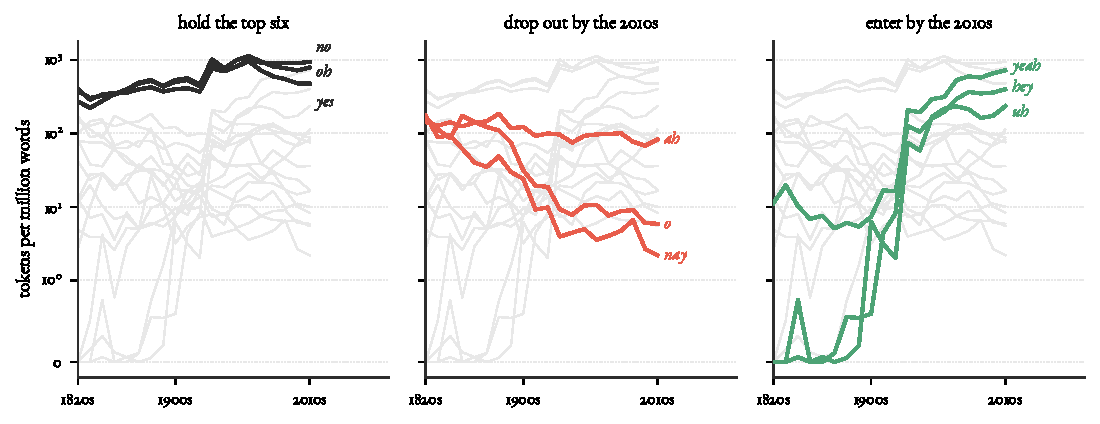
\includegraphics[width=\textwidth]{interjection-turnover.pdf}
  \caption{Turnover in the COHA interjection-tagged inventory. Each panel
  shows the twenty most frequent tagged lemmas across the corpus in grey,
  with one group highlighted. Three of the 1820s top six are displaced
  in that ranking by the 2010s. Frequencies per million words use a
  symmetric log scale retaining zeros. These rankings don't measure
  stability of a grammatical, semantic, or interactional profile.}
  \label{fig:turnover}
\end{figure}

The frequencies were extracted on 27 July 2026 and archived under
\path{analysis/hand-extracted/}. The 1820s ranking uses the complete
111-form tagged list for that decade, rather than restricting the
comparison to the all-period top twenty. This preserves a valid
comparison of ranks while leaving the separate question of what
the tag includes open to measurement audit.

\subsection{Withdrawn confirmatory interpretations}

The derivative study asked whether verbal uses recruited from
\mention{boo}, \mention{ooh}, \mention{shoo}, and \mention{wow}
retained source-associated content. The primary script assigned
semantic residue to every retained row instead of measuring it
independently. Its resulting success counts and intervals reproduce
that assignment. They don't test semantic persistence. A separate
97-row recode may supply narrower descriptive evidence if its
recorded provenance and coding are sound; it doesn't cover the
preregistered early windows adequately (Appendix~\ref{app:morphgain}).

Source-associated content would in any event differ from continued
expressive-category membership. \mention{The performance wowed us}
can describe an impressed response without making the conventional
use-conditional contribution of exclamatory \mention{wow!}. A valid
study of content continuity would bear on one historical relation.
It wouldn't by itself show that a verb retained membership in
\intj{sem} while changing its grammatical category.

The \mention{fie} study attempted to compare loss of interactional,
semantic, and syntactic properties. Its model input includes obvious
optical character recognition (OCR) substitutions for \mention{He}, coded as lacking all three
properties. Many other rows have prediction-derived notes without
established independent verification. The denominator
fails the stated eligibility rule. The archived curves and fitted
dates support neither ordered nor simultaneous linguistic erosion
(Appendix~\ref{app:fie}).

These failures constrain the claims the worked case can make.
The documented history of \mention{gee} remains evidence for that
route; the grammatical and semantic contrasts remain available
for their respective analyses. The failed corpus tests contribute
no independent confirmation of a general pattern of residual
meaning or property loss. The framework's distinctions explain
the scope of that failure; they don't compensate for it.

\section{The general consequence}\label{sec:discussion}

An inquiry-relative account goes beyond observing that different
questions invite different classifications. It requires the analyst
to say which objects are grouped, which distinctions the grouping
preserves, and what evidence supports its intended contribution.
For the interjection case, those requirements turn an undifferentiated
category dispute into several identifiable comparisons. They also
make unsupported proliferation visible.

\subsection{Pluralism with local failure conditions}

Some apparent conflicts disappear when the inquiries are separated.
Prenominal \mention{damn} can share expressive meaning with a
standalone sign while differing in grammatical distribution. Other
conflicts remain within an inquiry: the two analyses of complement-taking
\mention{damn} compete over its grammatical organization, and broad
versus narrow interactional groupings compete over useful coverage.
Pluralism doesn't resolve these disagreements in advance. It
identifies the evidence capable of resolving each.

The same discipline supplies failure conditions. A proposed grouping
can lack stable membership diagnostics, fail to preserve the claimed
contrast, or lose a comparison with a better alternative. A projected
property can fail in cases whose membership was established independently.
A historical explanation can lack the required source evidence.
Changing the inquiry after failure creates a different claim with
a different burden; it doesn't preserve the earlier claim's support.

The initial three classifications have no exemption. A broad
\intj{prag} may organize a domain while its subtypes perform most
of the inferential work. A semantic class may prove better expressed
as a broader category of expressives. A grammar-facing class may
retain unresolved exceptional cases. These are assessable limitations
of particular proposals, alongside the descriptive contrasts already
supported. The openness of the family permits new candidates under
the same conditions.

\subsection{Overlap, mechanisms, and category standing}

Overlap itself supplies neither privilege nor disqualification.
For common sign-type bearers, intersections are well-defined and
may support useful representation under incomplete observation.
Their value depends on the task and alternatives, including
representations of the separate memberships and their dependencies.
There's no automatic fourth category corresponding to the overlap
of grammar, meaning, and interaction, and no reason to prohibit
one from proving useful for a specified inquiry.

Categories needn't be statistically independent to do distinct
inferential work. A grammatical property can correlate strongly
with a prosodic one while each answers a different question.
Categories can also share causal mechanisms. One
historical process can affect several dimensions; several processes
can yield similar outcomes. Evidence for those relations belongs
to the causal account, rather than following from the number
of categories an analyst recognizes.

A causal network is one possible representation of these dependencies.
The representation would need independently identified variables and evidence
for the proposed links. Profile stability alone doesn't determine
their direction, and convergence alone doesn't show maintenance
or corrective control. The inquiry-relative account makes room
for such explanations while distinguishing them from the descriptive
and representational achievements that can precede them.

Gradience is likewise a separate question. A classification can
have graded membership, several sharply defined subtypes, or
unresolved cases caused by missing evidence. A prototype account
addresses typicality and similarity \citep{rosch1975,taylor2003};
an inquiry-relative assessment asks what contribution that organization
supports. Either a prototype or a categorical representation
can succeed for a specified purpose. The account doesn't
make fuzziness a necessary condition of pluralism.

The resulting position permits unequal judgments among classifications
without giving a discipline permanent priority. A grouping can
be well supported for one question, merely prospective for another,
and unhelpful for a third. Its range of success is an empirical
and explanatory matter. The familiar word \term{interjection}
marks the historical meeting point of the inquiries, while their
justification depends on the work each grouping can support.

\section{Conclusion}\label{sec:conclusion}

English interjections make a general problem of classification
visible. Grammar, expressive meaning, and interaction preserve
different relations among conventional signs. Phonological organization
and ancestry extend the comparison, while realizations and historical
changes require explicit links to sign-type classifications. Broader
social and processing classes can be relevant without becoming
interjection-specific categories. The family remains open because
inquiries can identify further defensible distinctions.

Category standing requires a stated bearer, grouping basis,
contribution, scope, and comparison with alternatives. Evidence
can support description, projection, economical representation,
or causal explanation to different degrees. The worked case
supports particular contrasts and a documented recruitment history;
its audited corpus attempts don't establish their intended
generalizations. This separation allows overlapping classifications
to be evaluated without demanding one privileged extension or
turning an investigator's purpose into sufficient justification.

\ifblind\else
\section*{Acknowledgements}

I compiled empirical material for the Wikipedia article \enquote{English
interjections}, of which I'm the primary author. This paper reanalyses
that material as a worked case for inquiry-relative classification.

The archived data and analysis code are available at
\url{https://github.com/BrettRey/interjections-hpc/tree/master}.
The appendices distinguish their retained descriptive contributions
from the confirmatory interpretations withdrawn after audit.
\fi

\clearpage
\begingroup
\setlength{\emergencystretch}{3em}
\printbibliography
\endgroup

\clearpage

\appendix

\section[Supplementary materials]{Supplementary materials: GloWbE conditioning analysis}
\label{app:conditioning}

\subsection{Data and measurement}

Frequency counts for 18 items were extracted from GloWbE \citep{daviesfuchs2015}: 1.9 billion words across 20 countries. The items are the 10 most frequent interjection-tagged forms (\mention{yes}, \mention{no}, \mention{oh}, \mention{yeah}, \mention{hi}, \mention{hey}, \mention{wow}, \mention{hello}, \mention{ah}, \mention{ha}), three regional forms (\mention{lah}, \mention{yaar}, \mention{haba}), semi-regional \mention{eh}, boundary items \mention{cheers} and \mention{bye}, and fillers \mention{um} and \mention{uh}. Core counts are tag-restricted; regional counts are raw strings because the tagger doesn't recognize the relevant uses. Neither measure identifies the three worked sign-type classifications independently.

Country is assigned to a page rather than a speaker. Assignment uses Google's region function: country domains provide a direct cue, but for \texttt{.com} and \texttt{.org} sites Google \enquote{relies on several heuristics, including 1) the IP address for the web server, 2) who links to that website, and 3) who visits the website} \citep[4]{daviesfuchs2015}. 

Davies and Fuchs themselves question \enquote{how well Google has correctly identified web sites by country}. The page list was seeded through Google searches for \enquote{hundreds of very high frequency 3-grams (three word strings)} from the Corpus of Contemporary American English (p.~4), anchoring the sampling frame to American frequency data. Country differences may reflect genre mix, internet ecology, and sampling alongside linguistic variation.

Automatic tagging adds another measurement layer. An overall error rate doesn't warrant comparisons if validity varies by country \citep{reynolds2026didcorpus}. Concordance coding estimates precision, the proportion of tagged hits that are genuine, not recall, the proportion of genuine tokens retrieved. Neither \mention{haba} nor \mention{yaar} receives an interjection tag. All 373 Nigerian \mention{haba} hits are tagged as common or proper nouns, with 65\% on a reading including the proper noun. The raw-string regional counts can overstate frequency while a tag-restricted query misses these forms entirely.

\subsection{Geographic distributions}

Regional concentration is clear in the raw strings: \mention{lah} occurs at 9.35 per million words in Malaysia and 6.72 in Singapore, and \mention{yaar} at 2.88 in Pakistan and 2.33 in India, with near-zero rates elsewhere. Nigeria's 373 \mention{haba} hits give an upper bound of about 9 per million. Inspecting hits, counting five spellings, and excluding Nigerian Pidgin, indigenous-language material, and duplicates, \textcite[69]{unuabonahdaniel2020} report 248 tokens, or 5.8 per million. The gap illustrates why raw strings and tagged counts aren't directly comparable.

Among the core items, \mention{ah} has the largest cross-country coefficient of variation (CV; standard deviation divided by mean), 0.71: Singapore's 60.42 and Jamaica's 53.16 per million are about eight times Kenya's 7.62. For \mention{yeah}, CV is 0.55 and the United States--Tanzania comparison is approximately 6:1 (103.78 versus 16.85). \mention{Yes} and \mention{no} have lower CVs, 0.21--0.22. The fillers \mention{um} and \mention{uh} have CVs of 0.61 and 0.76, and \mention{bye} has 0.61.

Bootstrap intervals resample the twenty observed country sections. They describe sensitivity to that resampling, not sampling uncertainty over all English-speaking communities: the sections aren't a random sample of such communities. The \mention{yes}/\mention{no} intervals lie below those of eleven of the thirteen other nonregional items, overlapping only \mention{hello} and \mention{ha}. This supports their comparatively low observed dispersion. 

The remaining marginal intervals overlap; that doesn't establish equal dispersion or settle pairwise differences. A ranking would require paired contrasts within resamples. Regional concentration is better represented by the counts: when a form is absent from eighteen sections, resampling can sharply alter the mean and CV. For \mention{lah}, the interval runs from 0.89 to 4.27.

\begin{figure}[ht]
  \centering
  % Crop the archived title/subtitle: its median label is misleading because
  % stat_summary is evaluated within each item facet, with one rate per country.
  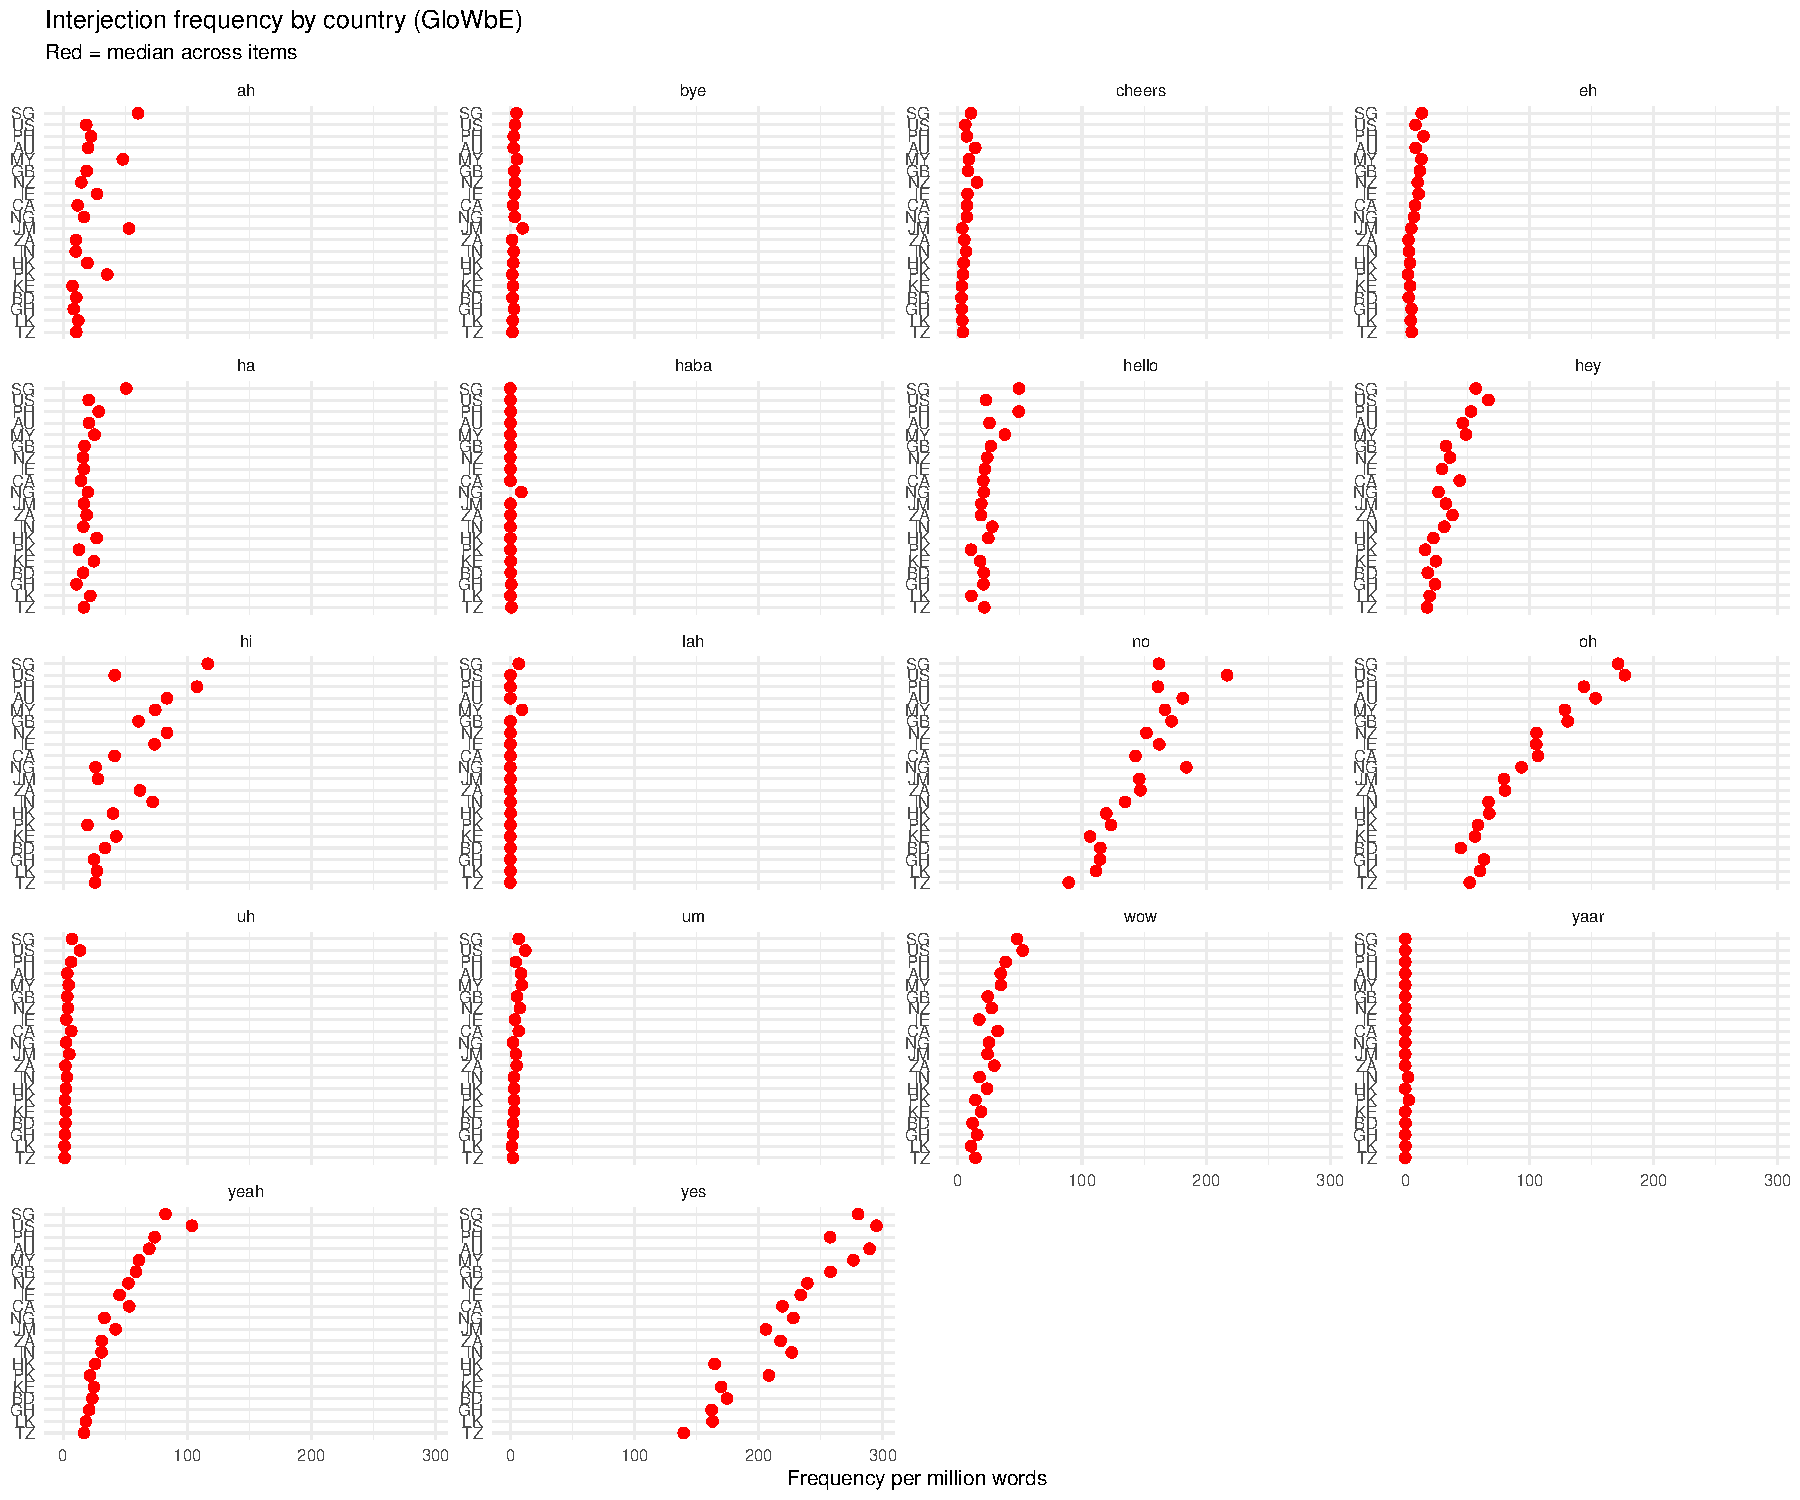
\includegraphics[width=\textwidth,trim=0 0 0 34,clip]{country-variation.pdf}
  \caption{Frequency per million words across 20 GloWbE country sections. Red points give the rate for each country--item combination. Regional strings (\mention{lah}, \mention{yaar}, \mention{haba}) concentrate in one or two countries; \mention{yes} and \mention{no} have comparatively low dispersion. Tagging and raw-string validity differ by item and country, as the audit below documents.}
  \label{fig:country-variation}
\end{figure}

\subsection{Concordance audit and sensitivity}

The tagger's training on inner-circle English limits its treatment of regional forms, but recognized items aren't necessarily clean. An initial twenty-token check of tagged \mention{ha} in Kenya and Tanzania retained six and eight interjections respectively; most other hits abbreviated \term{hectare} in agricultural and development prose. Applying the Kenyan estimate reduces 24.9 tokens per million to about 7.5 and moves Kenya from fifth to nineteenth among the twenty sections. This preliminary estimate differs from the fuller audit below.

The \mention{ha} audit also requires an explicit decision about laughter. Iterated \mention{HA! HA!} may represent laughter, closer to eye dialect than a lexical item, whereas sarcastic or sceptical \mention{ha} is an interjectional use. Written data make the distinction harder, and digital \mention{haha} may itself be conventionalized. This decision doesn't exclude imitative forms in principle; imitation is one proposed recruitment route. The reported counts include iterated laughter.

Coding tagged concordances across all twenty sections shows the sensitivity. Laughter constitutes 51.5\% of tagged \mention{ha} in the United States and 63.0\% in Great Britain. Across six defensible treatments of laughter and residual tokens, its CV ranges from 0.40 to 0.83 \citep[cf.][]{gelman2014statcrisis}; the reported 0.41 includes laughter. The dispersion measure depends on the criterion. A separate ranking result survives: country-specific validity correction moves Kenya from fifth to fifteenth under every coding.

The proportion of tagged \mention{ha} judged interjectional ranges from 34.5\% in Bangladesh to 84.0\% in Great Britain. \term{Hectare} dominates contamination in East Africa and South Asia; personal names matter in Singapore, where only 6.1\% of hits are \term{hectare}. Pooling country rates to reflect unequal precision~-- about 8,100 tagged tokens for the United States versus 420 for Ghana~-- moves no section by more than 0.6 percentage points. Between-section variation exceeds the sampling variation within sections. These checks correct false positives; they don't estimate missed interjections.

Spelling variants introduce another country-dependent error. Raw \mention{ya} and \mention{yeh} look like variants of \mention{yeah}, but they concentrate where substrate words are homographs: \mention{ya} peaks in Tanzania (19.5 per million) and Malaysia (13.9), and \mention{yeh} in Singapore (5.6), Pakistan (4.9), and India (4.9). No \mention{yeh} token carries the interjection tag. Pooling both strings with \mention{yeah} reduces its CV from 0.55 to 0.46 while importing non-English tokens unevenly, so the analysis keeps them separate.

Adding \mention{umm}, \mention{ummm}, and \mention{ummmm} to \mention{um} changes its CV from 0.61 to 0.60 with Pakistan excluded, but to 0.72 with Pakistan included. Pakistan returns nearly eight times as many \mention{umm} as \mention{um} tokens, against a median ratio of about a third elsewhere. In a twenty-token Pakistani sample, nineteen are the Arabic teknonym \mention{Umm}, as in \mention{Umm Salama}, from hadith or biographical material; the twentieth mentions the filler. Raw-string lengthening thus measures substrate homography as well as orthographic variation.

Regional forms face the same problem. Hand-coding sixty-nine \mention{yaar} hits puts the English-matrix rate at roughly 60\% in Pakistan and 65\% in India; other hits include Tamil \mention{yaar} \enquote{who}, names, and Roman-script Hindi or Urdu. The relevant twenty-token samples are too coarse for correction, but establish that raw rates are upper bounds. Raw \mention{yes}, \mention{no}, \mention{ha}, \mention{ah}, \mention{oh}, \mention{well}, \mention{right}, and \mention{like} likewise include clausal, quoted, discourse-marker, literary, or noisy uses. The audit establishes a measurement result: validity varies across countries, so pooled frequencies can conceal measurement differences alongside linguistic differences.

\subsection{Model specification}

Four Bayesian negative binomial models were fitted in \texttt{brms}~2.23 in R, with four chains of 2,000 iterations, including 1,000 warmup iterations. Models m0--m2 use exact reloo for leave-one-out cross-validation; exploratory m3 is assessed through Pareto-smoothed importance sampling (PSIS) diagnostics only.

\begin{quote}
\small \noindent\texttt{m0} (unconditional):\\ \texttt{count \textasciitilde{} 1 + offset(log(words\_m)) + (1~|~item)}

\noindent\parbox{\linewidth}{\texttt{m1} (conditioned):\\ \texttt{count \textasciitilde{} 1 + offset(log(words\_m)) +}\\ \texttt{(1~|~item) + (1~|~country)}}

\noindent\parbox{\linewidth}{\texttt{m2} (item type):\\ \texttt{count \textasciitilde{} 1 + item\_type + offset(log(words\_m)) +}\\ \texttt{(1~|~item) + (1~|~country)}}

\noindent\parbox{\linewidth}{\texttt{m3} (exploratory):\\ \texttt{count \textasciitilde{} 1 + item\_type + offset(log(words\_m)) +}\\ \texttt{(1~|~item) + (1~+~item\_type~||~country)}}
\end{quote}

The country intercept in m1 estimates an overall frequency shift across items, not an item-specific country effect. Model m3 adds country-varying slopes by item type, but the sparse type cells~-- semi-regional: 1 item; boundary: 2; filler: 2; regional: 3~-- provide little support for those slopes. Neither model estimates grammatical availability separately from preference or frequency of relevant occasions.

\subsection{Results}

Exact leave-one-out comparisons for the confirmatory models are:

\begin{center}
\begin{tabular}{lrr}
  \hline
  Model & ELPD diff & SE diff \\
  \hline
  m1 (conditioned) & 0.0 & 0.0 \\
  m2 (item type) & $-$9.3 & 7.9 \\
  m0 (unconditional) & $-$17.9 & 13.3 \\
  \hline
\end{tabular}
\end{center}

The country-conditioned model has the highest expected log predictive density (ELPD) point estimate, with an imprecise advantage over m0: $\Delta$ELPD = 17.9, standard error 13.3. Adding item type doesn't improve the point estimate. Model m3 isn't formally ranked because nine observations retain Pareto $k > 0.7$ after moment matching, leaving its PSIS estimates unstable.

In m1, the country standard deviation is 0.44 (95\% credible interval [CrI]: 0.28--0.65), against an item standard deviation of 2.07 (1.49--2.96), a ratio of 4.7:1. The country interval describes estimated variation under the model; its positive bounds aren't independent evidence against an absent effect, since standard deviations are constrained to be nonnegative. The predictive comparison and descriptive frequencies supply the relevant evidence. With 18 items $\times$ 20 countries = 360 observations, the ELPD uncertainty remains substantial.

To propagate the \mention{ha} precision estimates, each country's count was thinned by draws from its \textsc{beta} posterior, leaving the other seventeen items unchanged, and m0 and m1 were refitted. Within this sensitivity analysis, country standard deviation changes from 0.42 to 0.44 with iterated laughter included and 0.45 with it excluded; the model-comparison values change from 28.8 to 26.9 and 28.5. These approximate leave-one-out values support only an internal comparison, not replacement of the exact-reloo results above. Precision correction leaves recall unidentified.

The evidence supports geographic concentration of particular strings and additional overall country variation in these measured frequencies. It doesn't establish social indexing, item-type-specific conditioning, category-boundary decomposition, or a process maintaining the interjectional profile. The audit explains why those stronger interpretations require independently validated uses and comparable contexts.

\clearpage

\section[Semantic residue in COHA]{Supplementary materials: audit of the semantic-residue analysis in COHA}
\label{app:morphgain}

\subsection{Design and extraction}

The morphology-gain study was preregistered before confirmatory extraction and coding, after disclosed feasibility queries (\texttt{f1a2193}, 27 May 2026). Its fixed COHA source families were \mention{wow}, \mention{boo}, \mention{ooh}, and \mention{shoo}, over 1820--2019. The target derivatives were \mention{wowed}, \mention{wowing}, \mention{wows}; \mention{booed}, \mention{booing}, \mention{boos}; \mention{oohed}, \mention{oohing}, \mention{oohs}; and \mention{shooed}, \mention{shooing}, \mention{shoos}. Bare forms were excluded. Extraction on 27 May 2026 used key-word-in-context (KWIC) exports; chart requests for \mention{oohed} and \mention{oohing} failed, but their KWIC exports loaded. The extraction summary records minor chart/KWIC count discrepancies.

The go/no-go threshold required 20 analyzable derivatives and two decades with at least three each. The archived pipeline marked all families as passing the extraction threshold (GO):

\begin{center}
\begin{tabular}{lrrl}
  \toprule
  Family & Included tokens & Decades with 3+ & Status \\
  \midrule
  \mention{boo} & 364 & 10 & GO \\
  \mention{ooh} & 52 & 6 & GO \\
  \mention{shoo} & 410 & 13 & GO \\
  \mention{wow} & 143 & 9 & GO \\
  \bottomrule
\end{tabular}
\end{center}

\subsection{Intended measures and implementation}

The intended confirmatory measures were VP-head syntax and semantic residue: impressed or evaluative response for \mention{wow}, disapproval or contempt for \mention{boo}, appreciative or surprised response for \mention{ooh}, and directive away-sending for \mention{shoo}. Secondary codes concerned interactional residue~-- recognizable response, uptake, display, or direction~-- and a recoverable target, object, addressee, or stimulus.

An implementation audit changes the evidential status of the results. The archived primary-coding script first applies exclusion rules, then assigns both \texttt{verbal\_syntax = 1} and \texttt{semantic\_residue = 1} to every retained row. The exclusion rules were intended to select verbal uses; their accuracy can't be inferred from the syntax code automatically assigned to every retained row. The resulting file contains 1,462 rows: 969 included and 493 excluded. Semantic persistence wasn't independently measured in this primary coding pass; it was assigned by the pipeline. The outputs below don't constitute a confirmatory result.

Even independently established source content would need separating from expressive meaning type. A verb can describe or cause the response expressed by its source interjection without contributing use-conditionally itself. \mention{The performance wowed us} illustrates that distinction. Continuity of source-associated content would support a limited historical relation, not continued \intj{sem} membership.

\subsection{Archived outputs and their limits}

The confirmatory window began with the earliest decade containing at least three included derivatives and extended until it contained ten. Success required both confirmatory codes; the preregistered support rule placed the lower Jeffreys 95\% interval bound above 0.5. The pipeline produced:

\begin{center}
\begin{tabular}{lrlrrl}
  \toprule
  Family & Tokens & Window & $n$ & Assigned successes & Jeffreys 95\% CI \\
  \midrule
  \mention{boo} & 364 & 1920s & 17 & 17 & [0.865, 1.000] \\
  \mention{ooh} & 52 & 1960s--1980s & 10 & 10 & [0.783, 1.000] \\
  \mention{shoo} & 410 & 1890s--1900s & 16 & 16 & [0.857, 1.000] \\
  \mention{wow} & 143 & 1930s--1940s & 11 & 11 & [0.800, 1.000] \\
  \bottomrule
\end{tabular}
\end{center}

All four outputs meet the numerical rule because the semantic outcome was fixed for retained rows. The secondary diachronic model wasn't estimated because the assigned residue variable had no variation. These primary-pipeline records preserve the preregistered attempt; they establish neither semantic persistence nor a general tendency for interjections to acquire morphology or syntax.

\subsection{Reliability record and files}

The archived 10\% reliability sample contains 97 retained rows (seed 2026). Both comparison files are constant for inclusion, VP-head status, and semantic residue, so their agreement is 1.000 but Cohen's $\kappa$ is undefined. The reliability script instead returned 1.000 when expected agreement equalled one; that output isn't a valid $\kappa$. The sample also excludes rejected rows, so it doesn't audit false exclusions.

The archive contains a separate recorded recode, internally attributed to
Brett Reynolds as a blind human pass. Its secondary codes and notes differ
from the primary file, but the present implementation audit can't
independently verify the recorded human and blind provenance. If that
provenance and the coding rubric are sound, the sample can supply narrower
descriptive evidence of source-content continuity. Undefined $\kappa$
doesn't erase that possible contribution.

The recode covers only three of the 54 early-window rows used for the
confirmatory result: one each for \mention{boo}, \mention{shoo}, and
\mention{wow}, and none for \mention{ooh}. It can't replace
independent coding of the preregistered windows. The agreement table
records the comparison available in the archive, without treating it
as validation of the full primary dataset or of the claimed confirmation.


\begin{center}
\begin{tabular}{lrr}
  \toprule
  Code & Agreement & Cohen's $\kappa$ \\
  \midrule
  Inclusion & 1.000 & undefined \\
  VP-head status & 1.000 & undefined \\
  Semantic residue & 1.000 & undefined \\
  Interactional residue & 0.887 & 0.297 \\
  Targeted entity & 0.557 & 0.025 \\
  \bottomrule
\end{tabular}
\end{center}

The audit uses repository revision \texttt{074dfb44cef5b18d292ac176ba5acbfedc76e3b1}. Under \path{analysis/morphgain-confirmatory/}, the retained outputs are \path{morphgain-extraction-summary.csv}, \path{morphgain-go-nogo-summary.csv}, \path{morphgain-coding-summary.csv}, \path{morphgain-confirmatory-results.csv}, \path{morphgain-earliest-windows.csv}, and \path{morphgain-reliability-results.csv}. The corresponding scripts in \path{analysis/} are \path{morphgain-confirmatory-extract.mjs}, \path{morphgain-confirmatory-prepare.py}, \path{morphgain-confirmatory-code-primary.py}, \path{morphgain-confirmatory-analyze.py}, and \path{morphgain-confirmatory-reliability.py}. They document the implementation; they don't supply the missing independent semantic measurement for the full confirmatory dataset.

\clearpage

\section[Fie in COHA]{Supplementary materials: audit of the \mentionhead{fie} analysis in COHA}
\label{app:fie}

\subsection{Design, coding, and denominator}

The preregistration (\texttt{e18675b}, 15 March 2026) predicted interactional, then semantic, then syntactic loss among attested COHA uses of \mention{fie}, 1820--2019. It excluded metalinguistic mentions, non-English passages, metadata, and optical character recognition (OCR) noise. Represented speech, including fictional dialogue, was eligible. This ordered-erosion hypothesis was an additional historical commitment; it doesn't follow merely from distinguishing three worked sign-type classifications.

The archived analysis contains 616 coded rows. Its exclusion file separately records 141 entries: 134 OCR errors, three metalinguistic mentions, two non-English cases, and two name fragments. However, the model input still includes obvious OCR substitutions coded zero on all three diagnostics, including \enquote{FIe stroked his closed eyelids} (F014), \enquote{FIe drew her to him} (F028), and \enquote{FIe turned his attention} (F043). The model filters only for a non-missing syntactic code. Thus the stated exclusion rule wasn't successfully implemented in the analysed denominator.

The joint syntactic--semantic--interactional codes are 111 for 448 rows, 000 for 139, 011 for 19, 100 for eight, and 010 for two. In addition, 350 rows carry a note beginning \enquote{predicted}; the archive doesn't establish independent manual verification of all these assignments. These are implementation findings, not new linguistic classifications. An OCR substitution isn't an interjection that has lost three properties. The archived declines can't establish either ordered or simultaneous linguistic erosion.

\subsection{Archived agreement and proportions}

The decade column was hidden in the randomized coding sheet. The reported 10\% blind-recode comparison ($n = 62$) yielded:

\begin{center}
\begin{tabular}{lrr}
  \hline
  Diagnostic & Agreement & Cohen's $\kappa$ \\
  \hline
  \intj{syn} & 87.1\% & 0.68 \\
  \intj{sem} & 96.8\% & 0.90 \\
  \intj{prag} & 96.8\% & 0.90 \\
  \hline
\end{tabular}
\end{center}

These archived agreement values don't validate inclusion decisions or resolve the provenance of predicted codes. Figure~\ref{fig:fie-raw} likewise records the unvalidated input: proportions of 85--100\% through the 1890s, a decline between 1900 and 1940, and later fluctuations. Historical fiction and Shakespeare adaptations contribute positive represented uses in the 1980s and 2000s. Publication dates index the sampled texts, not necessarily the contemporary availability of the represented sign-type.

\begin{figure}[htbp]
  \centering
  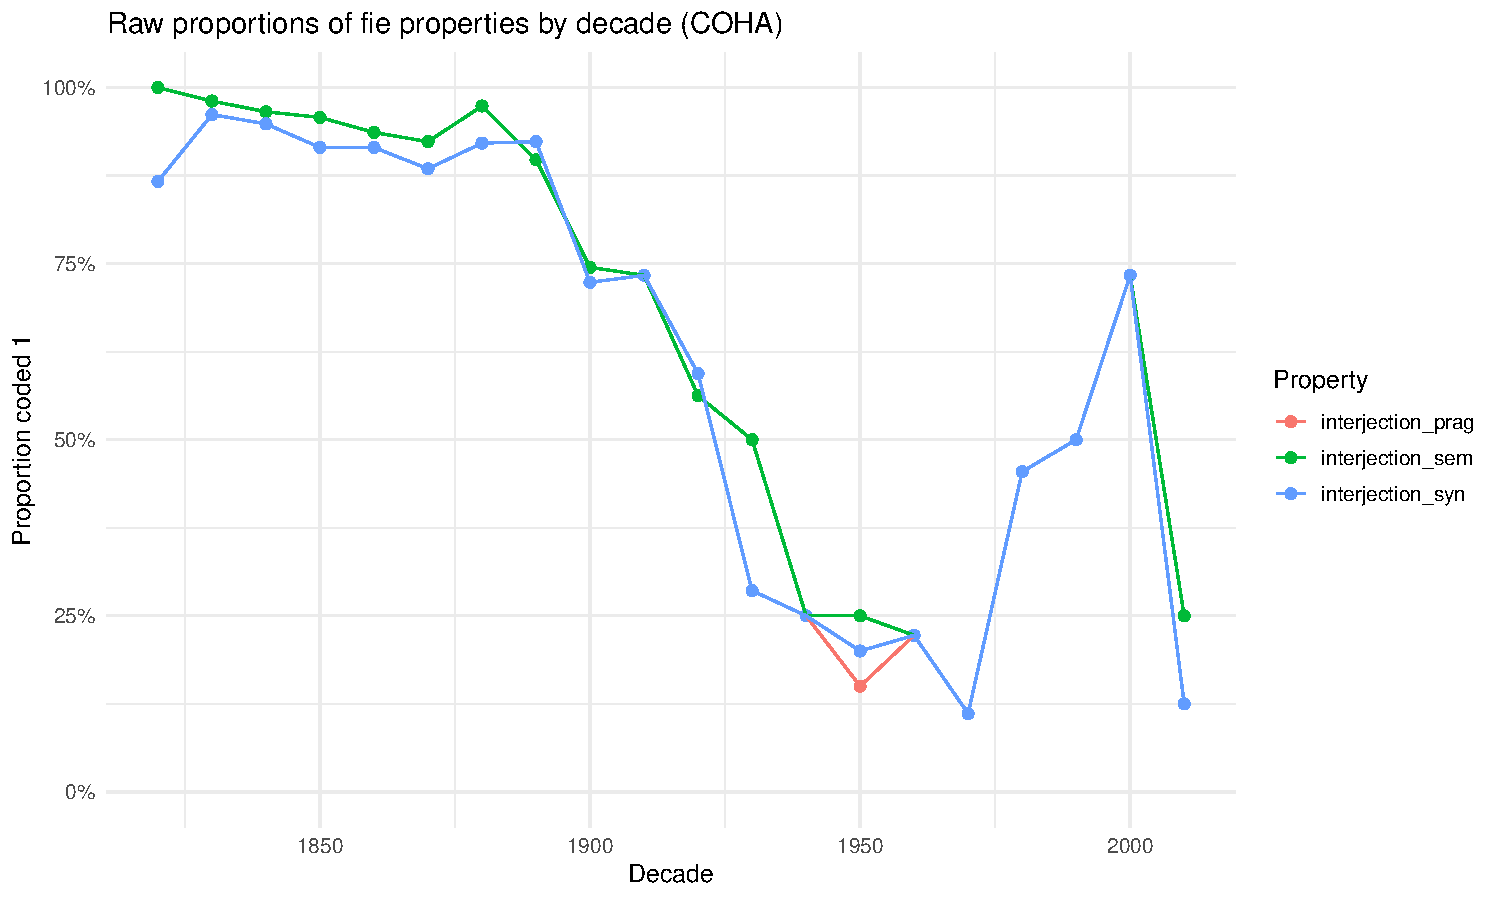
\includegraphics[width=.82\textwidth]{fie-raw-proportions.pdf}
  \caption{Archived proportions coded~1 by decade in the 616-row \mention{fie} input (COHA, 1820--2019). These are the original diagnostic trajectories, retained to document the attempted analysis. Because OCR substitutions remain in their denominator as zero-valued observations, the curves aren't interpreted as estimates of linguistic property loss.}
  \label{fig:fie-raw}
\end{figure}

\subsection{Archived models and interpretation}

The script fits three separate decade-level binomial logistic regressions, with time centred and scaled in ten-year units. Its normal priors have mean zero and standard deviations 1.5 for the intercept and 0.5 for the slope, with the latter restricted to negative values. Each fit uses four chains, 2,000 warmup and 2,000 subsequent iterations per chain, and seed 2026. The negative-slope restriction imposes monotonic decline and can't model revival. Separate likelihoods also leave the three outcomes' within-token dependence unmodelled.

The script centres decade labels rather than the midpoints specified in the preregistration. Because centring cancels a common offset, this discrepancy leaves the fitted predictor and the ordering probability unchanged. It shifts the conversion back to calendar dates by approximately five years. This bookkeeping issue is separate from the invalid denominator, which blocks the substantive interpretation.

\begin{samepage}
The reported ED50 dates ($\tau$, the 0.5 probability crossing) were:

\begin{center}
\begin{tabular}{lrr}
  \hline
  Diagnostic & $\tau$ (median) & 95\% CrI \\
  \hline
  \intj{syn} & 1947 & 1937--1958 \\
  \intj{prag} & 1948 & 1939--1959 \\
  \intj{sem} & 1949 & 1941--1960 \\
  \hline
\end{tabular}
\end{center}
\end{samepage}

The archived probability of $\tau_{\text{int}} < \tau_{\text{sem}} < \tau_{\text{syn}}$ is 0.13, below the preregistration's informal 0.25 threshold for \enquote{inconsistent}. Identical independent priors assign each strict ordering probability $1/6$, so 0.13 wouldn't itself be strong evidence against this order even with a valid denominator. Marginal interval overlap wouldn't establish equality or simultaneity either. More fundamentally, the measurement audit supersedes the substantive interpretation of all these outputs: they supply no present test for or against ordered erosion.

\begin{figure}[ht]
  \centering
  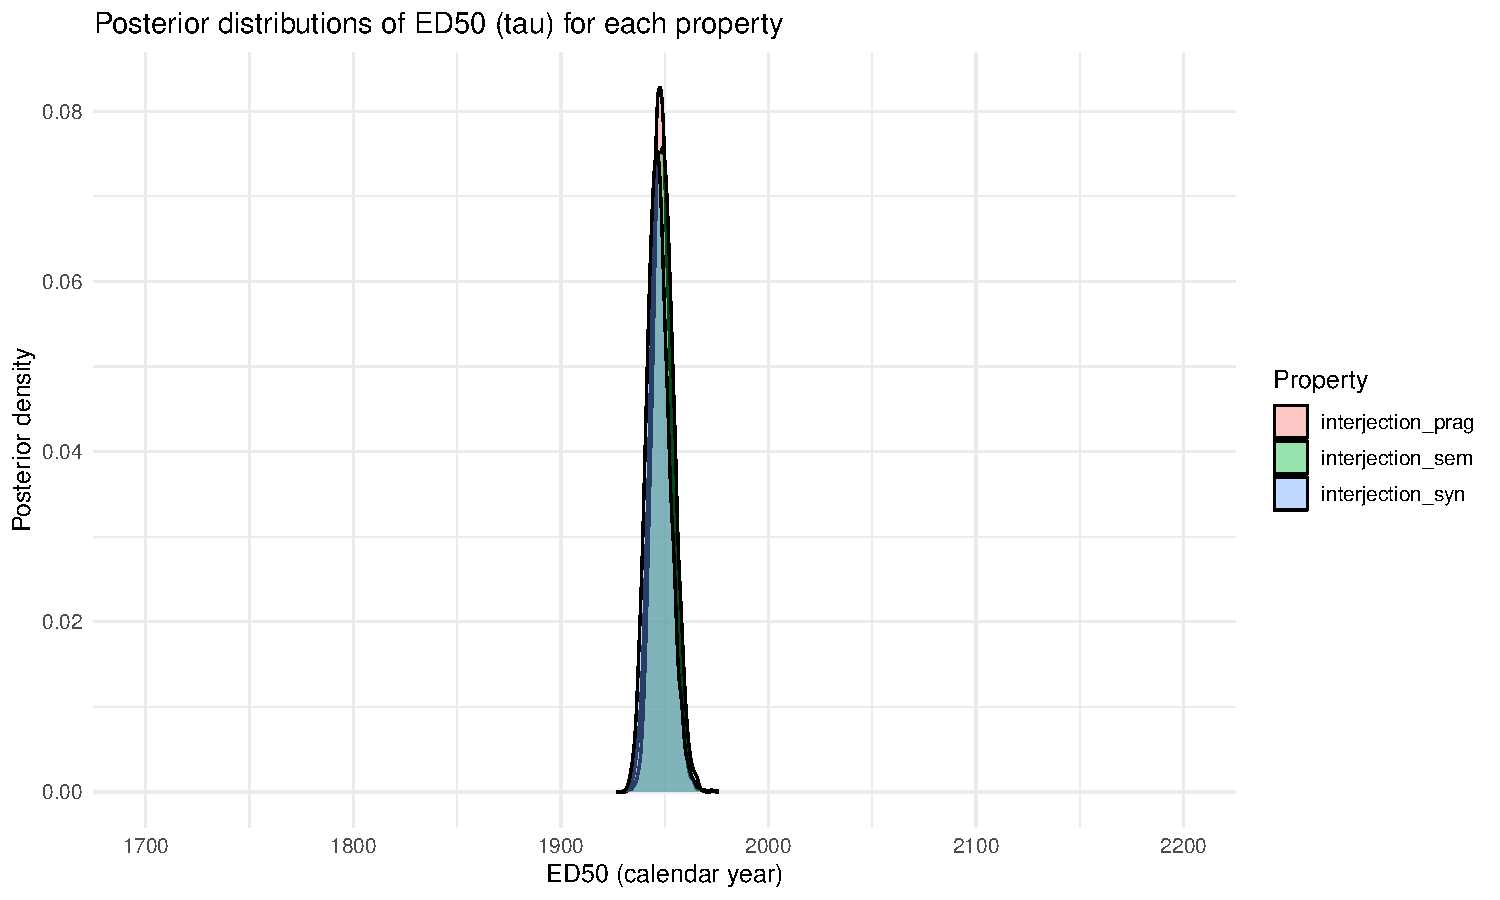
\includegraphics[width=.86\textwidth]{fie-tau-posteriors.pdf}
  \caption{Archived ED50 distributions from an analysis whose input failed the preregistered exclusion rule. The numerical outputs are retained for the audit record; their overlap isn't evidence for simultaneous loss, and the distributions aren't interpreted as valid estimates of linguistic erosion.}
  \label{fig:fie-tau}
\end{figure}

The audit is tied to repository revision \texttt{074dfb44cef5b18d292ac176ba5acbfedc76e3b1}, especially \path{fie-coha-preregistration.md}, \path{analysis/fie-confirmatory-model.R}, \path{analysis/fie-coding-sheet-annotated.csv}, and \path{analysis/fie-excluded.csv}. A valid comparison would first distinguish eligible occurrences from noise, then separate changing mixtures of sign-types from diagnostic change conditional on a bearer. No recoding or replacement model is reported here.

\end{document}
